\documentclass[
	12pt,                      % Schriftgrösse 12pt
	a4paper,                   % Layout für Din A4
	english,                   % neue deutsche Rechtschreibung nach der Reform
	oneside,                   % Layout für einseitigen Druck
	headinclude,               % Kopfzeile wird Seiten-Layouts mit berücksichtigt
	headsepline,               % horizontale Linie unter Kolumnentitel
	plainheadsepline,          % horizontale Linie auch beim plain-Style
	BCOR=12mm,                  % Korrektur für die Bindung
	DIV=18,                    % DIV-Wert für die Erstellung des Satzspiegels, siehe scrguide
	parskip=half,              % Absatzabstand statt Absatzeinzug
	openany,                   % Kapitel können auf geraden und ungeraden Seiten beginnen
	bibliography=totoc,        % Literaturverz. wird in und sonstige Verzeichnisse mit ins Inhaltsverzeichnis
	numbers=noenddot,          % Kapitelnummern immer ohne Punkt
	captions=tableheading,     % korrekte Abstaende bei TabellenUEBERschriften3
	]{scrbook}[2001/07/30]     % scrbook-Version mind. 2.8j von 2001/07/30

%##########################################################################################################
%
% Packete laden
%
%##########################################################################################################

\usepackage[english]{babel}
\usepackage[utf8]{inputenc}                    % Input-Encoding: ansinew for Windows
\usepackage[T1]{fontenc}                       % T1-kodierte Schriften, korrekte Trennmuster für Worte mit Umlauten
\usepackage{ae}                                % Für PDF-Erstellung

\usepackage[
	format=hang,
	font={footnotesize, sf},
	labelfont={bf},
	margin=1cm,
	aboveskip=5pt,
	belowskip=5pt,
	]{caption,subfig}                          % mehrzeilige Captions ausrichten; subfig: Untergrafiken
\usepackage{wrapfig}

\usepackage[centertags]{amsmath}               % AMS-Mathematik, centertags zentriert Nummer bei split
\usepackage{amssymb}                           % zusätzliche Symbole
\usepackage{trfsigns} 					       % für bestimmte Symbole
\usepackage{graphicx}                          % zum Einbinden von Grafiken
\usepackage[svgnames,table,hyperref]{xcolor}
\usepackage{float}                             % u.a. genaue Plazierung von Gleitobjekten mit H
\usepackage{epsfig}                            % eps Format für Grafiken
\usepackage[pdftex,pstarrows]{pict2e}
\usepackage{array}
\usepackage{listings}						   % Code-Einbindungsumgebung
\usepackage{courier}                           % verwende Courier statt cmtt als monospace-schrift
\usepackage{setspace}                          % Zeilenabstand einstellbar
\usepackage{rotating}
\onehalfspacing                                % eineinhalbzeilig einstellen
\usepackage{longtable}					       % Ermöglicht Tabellen die über den Seitenumbruch gehen (s. Symbolverzeichnis)
\usepackage{scrlayer-scrpage}
\usepackage{scrhack}                         % Kopf und Fusszeilen-Layout passt besser zur Dokumentklasse KOMA-Skript (scrbook) als das Pake fancyhdr, sonst ziemlich gleichwertig
\typearea[current]{current}                    % Neuberechnung des Satzspiegels mit alten Werten nach Änderung von Zeilenabstand,etc
\usepackage{xcolor,colortbl}                   % Packet um Tabellen bunt auszufüllen
\usepackage{wasysym}                           % Promillezeichen und co.
\usepackage{tabularx}
\usepackage{booktabs}
\usepackage{multirow}
\usepackage{braket}
\usepackage{algorithm}
\usepackage{algorithmic}
\usepackage{csquotes}
\usepackage{stix}           % changes all fonts !
\usepackage{wrapfig}

\usepackage{color, colortbl}
\definecolor{Gray}{gray}{0.9}

% use Tikz to draw graphics
\usepackage{tikz}
\usetikzlibrary{shapes,arrows}
\tikzstyle{decision} = [diamond, draw, fill=red!20,
text width=4em, text badly centered, node distance=1.7cm, inner sep=2pt]
\tikzstyle{block} = [rectangle, draw, fill=blue!20,
text width=10em, text centered, rounded corners, node distance=1.35cm, minimum height=2em]
\tikzstyle{line} = [draw, -latex']
\tikzstyle{cloud} = [draw, circle, text centered, fill=red!20, node distance=4cm,
minimum height=1.5em, text width=2em]


\usepackage[
	backend=biber,
	style=chem-angew,			% Style Angewandte Chemie
]{biblatex}     		 		% Biblatex Paket für Referenzen
\addbibresource{literatur.bib}	% File were you store sources

%##########################################################################################################
%
% PDF-Erzeugung: pdflatex statt latex aufrufen!
%
%##########################################################################################################

\pdfoutput=1
\usepackage[pdftex,  % muss letztes Package sein!
	pdftitle={Masterthesis},%
	pdfauthor={Andreas Hulm},%
	pdfsubject={free energy},%
	pdfkeywords={ ... },%
	pdfstartview={FitH},%
	pdfstartpage={5},%
	bookmarks,%
	raiselinks,%
	pageanchor,%
	hyperindex,%
	colorlinks,%
	citecolor=black!60!black,%
	linkcolor=black!70!black,%
	urlcolor=magenta!70!black,%
	filecolor=magenta!70!black,%
	menucolor=orange!70!black,%
    ]{hyperref}

%##########################################################################################################
%
% New- and Renew-Commands
%
%##########################################################################################################


\renewcommand{\headfont}{\normalfont\sffamily}             % Kolumnentitel serifenlos
\renewcommand{\pnumfont}{\normalfont\ttfamily\bfseries}    % Seitennummern typewriter und fett
\pagestyle{scrheadings}

% Einkommentieren falls beidseitige Darstellung erwünscht!!! aktuell definiert: oneside -> Layout fuer einseitigen Druck

%\ihead[]{\headmark}              % Kolumnentitel immer oben innen
%\ohead[\pagemark]{\pagemark}     % Seitennummern immer oben aussen
%\lefoot[]{}
%\rofoot[]{}                      % Seitennummern in der Fusszeile löschen

\newcommand {\jkarray}[1]{\ensuremath{\underline{#1}}}
\newcommand {\jkmatrix}[1]{\ensuremath{\underline{\underline{#1}}}}
\newcommand {\einheit}[1]{\ensuremath{\mathrm{\left[#1\right]}}}
\newcommand {\lived}[2]{($\ast$#1, $\dagger$#2)}  %

%###########################################################################################################
%
% Parameter für die jeweiligen Pakete definieren
%
%###########################################################################################################

\lstdefinestyle{cppcode}{language={[Visual]C++},%
	basicstyle=\ttfamily\footnotesize,%
	keywordstyle={\color{Navy} \bfseries},%
	identifierstyle={\color{DarkRed}},%
	commentstyle={\color{DarkOrange!50!black}\slshape},%
	stringstyle={\color{DarkGreen}},%
	showstringspaces=false,%
	backgroundcolor={\color{LightSkyBlue!40}},%
	columns=fixed,%
	keepspaces=true,%
	basewidth={0.55em},%
	frame=shadowbox,%
	rulesepcolor=\color{Gray},%
	breaklines=true,%
	numbers=left,%
	numberstyle=\tiny,%
	escapeinside={°(}{)°},%
	moredelim={[is][\bfseries]{°^}{^°}},%
	belowcaptionskip=0.5cm%
	}%

\lstdefinestyle{fort}{language={[95]Fortran},%
	basicstyle=\ttfamily\small,%
	keywordstyle={\color{Navy} \bfseries},%
	identifierstyle={\color{DarkRed}},%
	commentstyle={\color{DarkOrange!50!black}\slshape},%
	stringstyle={\color{DarkGreen}},%
	showstringspaces=false,%
	backgroundcolor={\color{LightSkyBlue!40}},%
	columns=fullflexible,%
	keepspaces=true,%
	basewidth={0.6em},%
	rulesepcolor=\color{Gray},%
	frame=shadowbox,%
	escapeinside={°(}{)°},%
	moredelim={[is][\bfseries]{°^}{^°}},%
	belowcaptionskip=0.5cm%
	}%


\lstdefinestyle{pseudocode}{basicstyle=\ttfamily\small,%
	columns=fixed,%
	keepspaces=true,%
	basewidth={0.55em},%
	frame=shadowbox,%
	backgroundcolor={\color{LightSkyBlue!40}},%
	rulesepcolor=\color{Gray},%
	escapeinside={°(}{)°},%
	moredelim={[is][\bfseries]{°^}{^°}},%
	belowcaptionskip=0.5cm%
	}%

\lstdefinestyle{maple}{%
	basicstyle=\sffamily\small\color{Red}\bfseries,%
	rulecolor=\color{Black},%
	columns=fixed,%
	keepspaces=true,%
	basewidth={0.55em},%
	frame=shadowbox,%
	numbers=left,%
	numberstyle=\tiny\color{Black},%
	numberblanklines=false,%
	rulesepcolor=\color{Gray},%
	breaklines=true,%
	breakautoindent=true,%
	backgroundcolor={\color{LightBlue!60}},%
	rulesepcolor=\color{Gray},%
	escapeinside={°(}{)°},%
	moredelim={[is][\bfseries]{°^}{^°}},%
	belowcaptionskip=0.5cm%
	}%

\lstdefinestyle{matlab}{language={Matlab},%
	basicstyle=\ttfamily\small,%
	keywordstyle={\color{Navy} \bfseries},%
	identifierstyle={\color{DarkRed}},%
	commentstyle={\color{DarkOrange!50!black}\slshape},%
	stringstyle={\color{DarkGreen}},%
	showstringspaces=false,%
	backgroundcolor={\color{LightSkyBlue!30}},%
	breaklines=true,%
	breakautoindent=true,%
	columns=fullflexible,%
	keepspaces=true,%
	basewidth={0.6em},%
	rulesepcolor=\color{Gray},%
	frame=shadowbox,%
	numbers=left,%
	numberstyle=\tiny\color{Black},%
	escapeinside={°(}{)°},%
	moredelim={[is][\bfseries]{°^}{^°}},%
	belowcaptionskip=0.5cm%
	}%

\lstdefinelanguage{Python}{
	basicstyle=\ttfamily\small,%
	keywordstyle={\color{Navy} \bfseries},%
 	keywords={typeof, null, catch, switch, in, int, str, float, self, boolean, throw, import,return, class, if ,elif, endif, while, do, else, True, False , catch, def, from, for},
 	identifierstyle=\color{black},
	comment=[l]{\#},
	commentstyle={\color{gray}\slshape},%
	stringstyle={\color{DarkGreen}},%
	backgroundcolor={\color{LightSkyBlue!30}},%
	breaklines=true,%
	breakautoindent=true,%
	columns=fullflexible,%
	keepspaces=true,%
	basewidth={0.6em},%
	rulesepcolor=\color{Gray},%
	frame=shadowbox,%
	numbers=left,%
	numberstyle=\tiny\color{Black},%
	escapeinside={°(}{)°},%
	moredelim={[is][\bfseries]{°^}{^°}},%
 	sensitive=false,
 	morecomment=[s]{/*}{*/},
	belowcaptionskip=0.5cm%
}

\graphicspath{{figs/}{bilder/}{plots/}}    % Falls texinput nicht gesetzt -> Bildverzeichnisse

% hier sind Worte zu definieren die in der Worttrennung falsch oder nicht erkannt werden!

\hyphenation{Post-pro-cess-ing--In-te-gral}


%###########################################################################################################
%
% Aufbau des Dokuments -> Einfügen der einzelnen Teile
%
%###########################################################################################################

% '''''''''''''''''''''''''''''''''''''''''''''''''''''''''''''''''''''
\newcommand{\sectionnumbering}[1]{%
	\setcounter{section}{0}%
	\renewcommand{\thesection}{\csname #1\endcsname{section}}}
% '''''''''''''''''''''''''''''''''''''''''''''''''''''''''''''''''''''

\newcounter{romanPagenumber} % neuen Seitenzähler als Variable definieren

\begin{document}
	\frontmatter

	\setheadsepline{0.0pt} 		  %Dicke der Trennlinie Kopfzeile - Text -> für Erklärung Änderungen ausschalten und erst ab Kurzzusammenfassung beginnen!

	\pagenumbering{Roman}         % romanische Nummerierung für die Deckblätter, Inhaltsverzeichnis und co.

	\begin{titlepage}
\begin{center}
{
%\fontsize{18}{18}\selectfont   % font Gr��e undefiniert-> es wird nur mit \text gearbeitet

\vspace*{-1.5cm}
\hfill \includegraphics*[width=3cm, keepaspectratio=true]{lmulogo.png}

\hrule                                 % horizontale Linie ein

\textsc{\LARGE Ludwig-Maximilians-University Munich}\\[2cm]

\textsc{\Large }\\[0.5cm]

\textsc{\Large Fakultät für Chemie and Pharmazie}\\[2.5cm]

\textbf{\LARGE Adaptive-Biasing Enhanced-Sampling Algorithms for the Efficient Calculation of Free Energy Curves in Collective-Variable Space} \\[0.5cm]

\textsc{\Large Masterarbeit aus dem Fachbereich Theoretische Chemie}\\[2.0cm]

%\textsc{AK Ochsenfeld}\\[2.0cm]

\textsc{von}\\
\textsc{B.Sc. Andreas Valentin Hulm} \\[1,5cm]
\textsc{geboren am 29.04.1997} \\
\textsc{in Freising} \\ [2,5cm]

%\textsc{Für die Masterprüfung in Chemie an der} \\
%\textsc{\textbf{Ludwig-Maximilians-University Munich}}\\[2cm]

Beginn der Masterarbeit: 02.10.2020 \\
Masterarbeit beim Prüfungsamt eingereicht am: \today
}
\end{center}

\end{titlepage}
%\thispagestyle{empty}     % 2. Seite leer!
%\section*{}
     % Deckblatt Titel
	
\begin{titlepage}

\begin{center}

{\fontsize{14pt}{14}

\textsc{Master Thesis in Theoretical Chemistry} \\
\vspace{0.5cm}
\textsc{submitted to the LMU Munic}\\
\vspace{0.5cm}
\textsc{at the Department of Chemistry}\\
\vspace{0.5cm}
\textsc{}\\[3cm]

\textsc{\Large  \underline{Subject:}}\\[3.0cm]

\textbf{\Large Advanced enhanced sampling algorithms for free Energy calculation in collective variable space}\\[6cm]
}
{\fontsize{12pt}{12} \selectfont%
\begin{tabular}{ll}
Verfasser:& Andreas Valentin Hulm \\
Matrikelnummer:& 11353987\\
Referent:& Prof. Dr. Christian Ochsenfeld\\
Betreuer:& Dr. Johannes Dietschreid\\[1cm]
Begonnen am:& October 02, 2020\\
Eingereicht:& \today\\
Abschließend beurteilt am:&   \hspace{4cm} Note: \\
\end{tabular}
}
\end{center}

\end{titlepage}
     % Erklärung

	\chapter{Danksagung}
Mein Dank gilt Herrn Prof. Ochsenfeld für die Betreuung der Masterarbeit, sowie für hilfreiche Anregungen.
Desweiteren möchte ich mich bei Frau Prof. de Vivie-Riedle für die Übernahme der Zweitgutachtens bedanken.
Besonderer Dank gilt außerdem Dr. Johannes Dietschreit für die freundliche und konstruktive Unterstützung während der gesamten Arbeit, sowie allen Mitgliedern des AK Ochsenfeld für anregende Diskussionen.
Zuletzt möchte ich meiner Familie für ihren immerwährenden Rückhalt in besonders herausfordernden Zeiten danken.

	\addchap{List of Abbreviations}
\markboth{List of symbols}{List of symbols}
\label{cha:symbols}

\begin{longtable}[l]{lcp{10cm}}
	ABF		&&  Adaptive-biasing force method \\
	CV    &&  Collective variable \\
	CZAR  &&  Corrected z-averaged restraint estimator \\
	DFT   &&  Density functional theory \\
	eABF  &&  Extended adaptive-biasing force method \\
	HPC   &&  High performance computing \\
	FES   &&  Free energy surface \\
	MC    &&  Monte-Carlo simulation \\
	MD    &&  Molecular dynamics simulation \\
	meta-eABF && Metadynamics plus extended adaptive biasing force method \\
	MM    &&  Molecular mechanics \\
	MtD   &&  Metadynamics \\
	MW    &&  Multiple-walker strategy \\
	PES   &&  Potential energy surface \\
	PMF   &&  Potential of mean force \\
	QM    &&  Quantum mechanics \\
	TI    &&  Thermodynamic integration \\
  US    &&  Umbrella sampling \\
	WHAM  &&  Weighted histogram analysis method \\
	WTM   &&  Well-tempered metadynamics \\
	WTM-eABF && Well-tempered metadynamics plus extended adaptive biasing force method \\
\end{longtable}


	\setheadsepline{0.5pt}
	\tableofcontents              % Inhaltsverzeichnis
	\clearpage
	\setcounter{romanPagenumber}{\value{page}} % eigener Seitenzähler erhält aktuelle römische Seitenzahl

	\mainmatter                   % den Hauptteil beginnen
	\pagenumbering{arabic}        % ab hier wieder arabische Nummerierung

	\chapter{Introduction}
\label{cha:introduction}
Free energy differences are the driving force of chemical processes at or near thermodynamic equilibrium and therefore the central quantity that determines the behavior of these systems.\autocite{chipot2007free}
However, the calculation of free energies still constitutes one of the major challenges of computational chemistry.\autocite{kastner2011umbrella}
This is because free energy contains entropy, which is a measure for the available space of a system.
For more than a few atoms, mapping available space requires extensive sampling, making free energy calculations computationally exceedingly demanding.\autocite{kollman1993free}
Therefore, although the statistical-mechanical foundations for the calculation of free energy curves were laid decades ago,\autocite{chipot2007free} it is only in recent years that increasing computational power combined with major advances in the efficiency of quantum-mechanical/molecular-mechanical (QM/MM) codes\autocite{ochsenfeld2007linear,shao2015advances,acun2018scalable} made their application possible.
Today free energy calculations are frequently used in several important areas ranging from biochemistry\autocite{gumbart2013standard,fu2017new,capelli2019chasing}, to pharmacology\autocite{yu2017computer,sinko2013accounting} or
nanotechnology.\autocite{fu2017lubricating,chen2019tumbling}

In practice to sample configurations of chemical systems time trajectories are calculated by means of molecular dynamics (MD) or Monte-Carlo (MC) simulations.\autocite{ponder2003force,burke2012perspective}
However, as most chemical reactions involve crossing of free energy barriers, reaction coordinates often constitute slow degrees of freedom.
This means that trajectories stay kinetically trapped in \textit{metastable} states, e.g., the educt or product state, and are unable to explore the full reaction coordinate.\autocite{chipot2007free}
%Simple trajectories are therefore poorly suited for sampling of reaction coordinates.\autocite{chipot2007free}
To address this problem the vary active research field of \textit{enhanced sampling} emerged, which has already produced numerous different approaches to speed up exploration of reaction coordinates.
\autocite{jiang2010free, sugita1999replica,den2000thermodynamic, ciccotti2005blue, barducci2008well}

One particular successful class of algorithms relies on the definition of \textit{collective variables} (CVs).
This variables need to distinguish between the educt and product states, while ideally capturing all slow degrees of freedom along the way.\autocite{fiorin2013using}
Typically maximal two dimensional variables are chosen, because of the massive growth of computational cost of sampling in higher dimensional space, also known as \textit{curse of dimensionality}.\autocite{koppen2000curse}
The potential energy or forces along the CVs are then altered in a way, that increases the time spent in important regions.
One of the oldest and most widespread approaches is \textit{Umbrella Sampling}\autocite{kastner2011umbrella}, where bias potentials along the reaction coordinate drive a system from the reactant to the product state.
The intermediate steps are covered by a series of windows, in each of which a MD simulation is performed.
From this simulations the full free energy curve can be calculated by combining all windows with the weighted histogram analysis method (WHAM).\autocite{kumar1992weighted}
This approach enables efficient sampling along the reaction coordinate due to parallelisation.
However, it also requires some knowledge of the free energy curve prior to simulation in order to adequately choose the bias potentials.
In addition, setting up and analyzing multiple MD simulations requires huge computer resources and is time consuming.

To address both shortcomings this thesis will focus on another class of enhanced sampling algorithms, termed \textit{adaptive biasing} methods.\autocite{barducci2008well,comer2015adaptive,lesage2017smoothed}
Here a time-dependent, self-learning bias potential or force is introduced, that evolves during the simulation to encourage uniform sampling along the CV.
One can think of two complementary approaches to build time-dependent biases:
The first one, e.g., \textit{metadynamics} (MtD)\autocite{barducci2011metadynamics} and its variants, encourages sampling by flooding valleys of the free energy landscape with a time-dependent potential.
Because of its simplicity and straightforward implementation it has been integrated in almost all popular MD engines and was broadly utilized for a large variety of problems.\autocite{vymetal2011gyration,tanida2020alchemical,ikeda2005hydration}
The second one, termed \textit{adaptive biasing force} (ABF)\autocite{comer2015adaptive} method, flattens the free energy landscape by application of a time-dependent bias force.
Despite its outstanding stability and beneficial formal convergence properties, the practical implementation and application of ABF has been thwarted by the analytical formulation of the biasing forces, thereby limiting the scope of the numerical scheme.\autocite{fiorin2013using}
Recently this limitations could been lifted by extended-Lagrangian based methods, where a fictitious particle is coupled to the CV.
In this framework the bias force used for enhanced sampling only acts on the fictitious particle, which renders its implementation trivial.
The resulting extended-system ABF (eABF)\autocite{lesage2017smoothed} method combines the wide applicability of MtD with the convergence properties of ABF.
Additionally the calculation of free energy curves can be separated from sampling acceleration with an asymptotically unbiased free energy gradient estimator, termed \textit{corrected z-averaged restraint} (CZAR).\autocite{lesage2017smoothed}
The resulting flexibility in the choice of bias force can be used to combine both metadynamics and ABF to well-tempered metadynamics extended-system ABF (WTM-eABF),\autocite{fu2018zooming,fu2019taming} a highly potent enhanced-sampling scheme, which stands out due to its efficiency and robustness.

In this thesis all aforementioned adaptive biasing algorithms are combined with highly efficient QM/MM calculations in the in-house FermiONs++\autocite{kussmann2013linear} program package, to enable the broad application of free energy calculations for large molecular systems at accurate level of theory.

	\chapter{Theoretical Background}
\label{cha:theory}

\section{Statistical thermodynamics and Free Energy}
\label{sec:freeE}

The formulation of the problem of free energy estimation starts with the Hamiltonian
\begin{equation}
  \textbf{H}(\textbf{x},\textbf{p})=\sum_{i=0}^{N}\frac{p_{i}^{ 2}}{2 m_i} + U(\textbf{x})
  \label{eq:lagrangian}
\end{equation}
of an arbitrary chemical system, where $(\textbf{x},\textbf{p})$ denotes a point in the phase space of the N-particle system of interest with atomic coordinates $\textbf{x}=(x_1, ..., x_N)$, momenta $\textbf{p}=(p_1,...,p_N)$ and masses $(m_1,...,m_N)$. $U(\textbf{x})$ is the potential energy given by any quantum chemical method or force field. If the canonical (N,V,T)-ensemble of such a system is sampled, for example by means of Langevin dynamics or Monte Carlo simulations, the probability distribution $\rho(\textbf{x})$ in the configuration space $\textbf{x}$ follows the Boltzmann distribution
\begin{equation}
  \rho(\textbf{x})=\frac{e^{-\beta U(\textbf{x})}}{\int e^{-\beta U(\textbf{x})} d\textbf{x}}=Z^{-1}e^{-\beta U(\textbf{x})}
  \label{eq:boltzmann}
\end{equation}
were $Z$ denotes the \textit{canonical partition function} and $\beta=(k_B T)^{-1}$ the inverse temperature with Boltzmann constant $k_B$.\autocite{chipot2007free}
%By acting as normalization constant to ensure $\int\rho(x)dx=1$, the partition function is the central quantity of statistical thermodynamics, relating macroscopic thermodynamic quantities to the microscopic details of a system.
In this thesis we will focus on alchemical transformations, $A\longrightarrow B$, which are represented by a small set of collective variables (CV's)
\begin{equation}
 \xi_1(\textbf{x}) : \mathbb{R} ^{3N} \to \mathbb{R}, ..., \xi_n(\textbf{x}) : \mathbb{R} ^{3N} \to \mathbb{R}
\end{equation}
that are sufficient to distinguish between key states of interest.
In this framework the probability distribution can be expressed by
\begin{equation}
  \rho(\xi)=\int \delta[\xi'(\textbf{x})-\xi]\rho(\textbf{x})d\textbf{x}=\braket{\delta [\xi'(\textbf{x})-\xi]}_\xi
  \label{eq:rho}
\end{equation}
where $\braket{}_\xi$ denotes the $\xi$-conditioned marginal distribution. The Helmholtz free energy $A$, i.e. potential of the canonical ensemble, is defined as
\begin{equation}
  A(\xi) = -\beta^{-1}\ln \rho(\xi)
  \label{eq:free energy}
\end{equation}
Note that the shape of the obtained free energy surface (FES) is not gauge invariant against the choice of CV function $\xi$. This is, however, no concern in the calculation of free energy differences, because the CV dependent feature is integrated out to obtain the probability that the system occupies state A or B.\autocite{bal2020free}
\begin{equation}
  \Delta A_{A\rightarrow B} = -\beta^{-1}\ln \frac{\int_B \rho(\xi)d\xi}{\int_A \rho(\xi)d\xi}=-\beta^{-1}\ln \frac{p_B}{p_A}
  \label{eq:free energy diff}
\end{equation}
However, in computer simulations the direct phase-space integrals used in equation \ref{eq:boltzmann} and \ref{eq:rho} are impossible to calculate.\autocite{chipot2007free} Instead the time average $P(\xi)$ is computed by monitoring $\xi$ during the simulation.
\begin{equation}
  P(\xi)=\lim_{t\rightarrow \infty}\frac{1}{t} \int_0^t \rho[\xi (t')] dt'
  \label{eq:ergodic}
\end{equation}
In practice, $P(\xi)$ is approximated as a histogram along the reaction coordinate with bins of fixed size.
Assuming that the system at hand behaves \textit{ergodic}, i.e. every point in phase space is visited during a infinitely long simulation, the ensemble average $\rho(\xi)$ converges to the time average $P(\xi)$ of one system.
However, transitions of high energy barriers during chemical reactions are typically rare events, that might happen on timescales far beyond what is feasible to compute, especially on accurate quantum chemical level of theory. Therefore most processes, for example in biochemical context, behave \textit{quasinonergodic}.
The problem of calculating accurate free energy differences hence really consists in adequate sampling of regions with high free energy (transition states) along the reaction coordinate.

For this purpose several \textit{enhanced sampling} algorithms were proposed.\autocite{jiang2010free, sugita1999replica,den2000thermodynamic, kastner2011umbrella, ciccotti2005blue, barducci2008well}
In this work we will focus on CV-based approaches, that alter the potential energy $U(\textbf{x})$ of the system in a way, that increases the time spent in important regions of configuration space during a simulation. One of the oldest and simplest methods to achieve the same is \textit{Umbrella Sampling} (US)\autocite{kastner2011umbrella}, which will be introduced in the following section.
The main focus of this work lies on \textit{Adaptive Biasing Methods} \autocite{barducci2011metadynamics,comer2015adaptive, lesage2017smoothed}, which aim for uniform sampling along the reaction coordinate by an history dependent biasing term (section \ref{sec:adaptive biasing}).
\newpage

\section{Umbrella Sampling (US)}
In its most common form US introduces a fixed harmonic bias potential of the form
\begin{equation}
  U_i^B(\xi) = \frac{k_i}{2}(\xi(t)-\xi_i)^2 \label{eq:US bias}
\end{equation}
where the index i indicates a given bias window along the reaction coordinate with force constant $k_i$.\autocite{kastner2011umbrella} From simulations in window i the biased probability distribution $P_i^B(\xi)$ is obtained
\begin{equation}
\begin{split}
  P_i^B(\xi) &= \frac{\int d\textbf{x} e^{-\beta (U(\textbf{x})+U_i^B(\xi(\textbf{x})))}\delta[\xi'(\textbf{x})-\xi]}
  {\int d\textbf{x} e^{-\beta (U(\textbf{x})+U_i^B(\xi(\textbf{x})))}} \\
             &= \frac{e^{-\beta U_i^B(\xi(\textbf{x}))}}{\int e^{-\beta (U(\textbf{x})+U_i^B(\xi(\textbf{x})))}d\textbf{x}} \int d\textbf{x} e^{-\beta U(\textbf{x})}\delta[\xi'(\textbf{x})-\xi]
\end{split}
\end{equation}
where $Z_B$ denotes the partition function of the biased potential energy $U(\textbf{x})+U_i^B(\xi(\textbf{x}))$.
Using equation \ref{eq:boltzmann} and \ref{eq:rho} the connection of $P_i^B$ to the unbiased probability distribution $P_i^0$ can be derived.
\begin{equation}
\begin{split}
  P_i^0(\xi) &= P_i^B(\xi)e^{\beta U_i^B(\xi)}\frac{\int e^{-\beta (U(\textbf{x})+U_i^B(\xi(\textbf{x})))}d\textbf{x}} {\int e^{-\beta U(\textbf{x})}d\textbf{x}} \\
  &= P_i^B(\xi)e^{\beta U_i^B(\xi)}\frac{Z_B}{Z_0}
\end{split}
\end{equation}
Inserting into equation \ref{eq:free energy} gives the unbiased free energy
\begin{equation}
  \begin{split}
  A_i(\xi) &= -\beta^{-1}\ln P_i^B(\xi) - U_i^B(\xi) - \beta^{-1}\ln\frac{Z_B}{Z_0} \\
           &= A_B(\xi) - U_i^B(\xi) - F_i \label{eq:A US}
  \end{split}
\end{equation}
The last therm of equation (\ref{eq:A US}) is the free energy difference between the unbiased and biased system. Since it is a constant it can be ignored in the calculation of free energy differences from a single window.

However, in order to enhance sampling along the reaction coordinate usually a stratification strategy is applied simulating multiple overlapping windows. In this case the global unbiased distribution of all combined windows is calculated with the \textit{Weighted Histogram Analysis Method} (WHAM).\autocite{kumar1992weighted} The goal of WHAM is to choose the weights $p_i(\xi)$ in order to minimize the statistical error of the global probability distribution of S combined windows
\begin{equation}
  P^U(\xi)=\sum_i^{S} p_i(\xi)P_i^0(\xi)
\end{equation}
under the constraint $\sum p_i = 1$. This is achieved by the iterative solution of the self-consistent WHAM equations
\begin{equation}
  p_i(\xi) = \frac{N_i \e^{-\beta_i U_i^B(\xi)+\beta_i F_i}}{\sum_j^S N_j \e^{-\beta_j U_j^B(\xi)+\beta_j F_j}} \label{eq:WHAM 1}
\end{equation}
\begin{equation}
  \e^{-\beta_i F_i} = \int P^U(\xi)\e^{-\beta_i U_i^B (\xi)}d\xi
  \label{eq:WHAM 2}
\end{equation}
where $F_i$ enters equation (\ref{eq:WHAM 1}) and $P^U$ enters equation (\ref{eq:WHAM 2}). $N_i$ is the number of samples collected in window i.
The biggest advantage of this approach is that all windows can be simulated in parallel on different computing nodes and only have to be combined once to solve the WHAM equations. This way extensive sampling of the reaction coordinate can be obtained efficiently.
However, the biasing potentials have to be chosen manually for each window, requiring some knowledge of the free energy surfaces at hand prior to the simulation.
Additionally, up to 50\% of the simulation time can be spent in overlapping regions of ascending windows.\autocite{comer2015adaptive}
In the next section we will look at different approaches, that eliminate both drawbacks by replacing equation \ref{eq:US bias} with an time dependent term, which evolves during the simulation to achieve uniform sampling of the reaction coordinate.

\newpage
\section{Adaptive Biasing Methods}
\label{sec:adaptive biasing}

Instead of dividing the reaction coordinate in several windows, with adaptive biasing methods the free energy can be estimated from one single simulation. For this purpose the systems dynamics are biased towards states corresponding to large values of the free energy along the transition coordinate via a history-dependent biasing potential. In contrast to other importance sampling strategies like umbrella sampling, this methods require less knowledge of the free energy surface at hand prior to the simulation, because the bias is not chosen manually. Instead, the biasing potential automatically adapts during the simulation to enable diffusive behavior along the transition coordinate.\autocite{comer2015adaptive, barducci2011metadynamics}

There are multiple adaptive biasing methods available, only differing in the construction of the bias. Potential based methods like metadynamics (MtD) disfavor already visited states by accumulating repulsive potentials along the CV (section \ref{sec:metaD}), while adaptive biasing force (ABF) methods compensate the mean force along the reaction coordinate to obtain uniform sampling (section \ref{sec:ABF}). Finally, as discussed in section \ref{sec:eABF}, using an extended Lagrangian, the technical requirements of ABF can be lifted without loosing its rigorous convergence behavior.\autocite{lesage2017smoothed} Additionally, this framework enables the combination of repulsive Mtd-potentials with ABF (meta-eABF/WTM-eABF), to unite the benefits of both approaches.\autocite{fu2018zooming,fu2019taming}

Although not necessary, stratification can increase the convergence of all adaptive biasing methods significantly. However, in contrast to US simulations, no WHAM and hence no overlap between ascending windows is required. For example in ABF simulations the global PMF can be recovered by simply joining the force estimates of all simulations.\autocite{comer2015adaptive} Multiple-Walker strategies can also be trivially implemented, by letting more than one simulation contribute to the same biasing potential, as will be discussed in section \ref{sec:MW}.\autocite{minoukadeh2010potential}

In principle adaptive biasing methods only rely on sampling of the canonical ensemble, which will be obtained using Langevin dynamics in this work. However, all methods can also be applied in combination with other MD or MC engines. A schematic procedure of adaptively biased Langevin dynamics is given in Algorithm \ref{alg:ABM}.

\begin{algorithm}[H]
  \caption{Velocity Verlet integrator for adaptively biased Langevin dynamics with atomic masses $\textbf{M}$, coordinates $\textbf{x}(t)$, momenta $\textbf{p}(t)$, potential $U(\textbf{x}(t))$, forces $F(\textbf{x}(t))$ and friction coefficient $\gamma$,}
  \label{alg:ABM}
    \begin{algorithmic}
      \WHILE{$t < t_{end}$}
        \STATE
        \STATE $\textbf{p}(t+\frac{1}{2}\Delta t) \leftarrow \textbf{p}(t) + \frac{1}{2} \bigl(F(\textbf{x}(t))dt-\gamma \textbf{M}^{-1}\textbf{p}(t) dt + \sqrt{2\gamma\beta^{-1}}dW_t \bigr)$
        \STATE $\textbf{x}(t+\Delta t) \leftarrow \textbf{x}(t) + \frac{2}{2+\gamma dt}\textbf{M}^{-1} \textbf{p}(t+\frac{1}{2}\Delta t) dt$
        \STATE /* Langevin dynamics
        \STATE
        \STATE $F(\textbf{x}(t+\Delta t)) \leftarrow -\nabla U(\textbf{x}(t+\Delta t))$
        \STATE /* get physical QM/MM forces
        \STATE
        \STATE $\xi \leftarrow f(\textbf{x}(t+\Delta t))$
        \STATE /* Calculate reaction coordinate from Cartesian coordinates
        \STATE
        \IF{$\xi_{min}\leq\xi\leq\xi_{max}$}
          \STATE
          \STATE $F_{B}(\xi, t+\Delta t))\leftarrow F_{B}(\xi, t))+\Delta F_{B}(\xi,t+\Delta t))$
          \STATE /* update history dependent bias force along reaction coordinate incrementally
          \STATE
          \STATE $F(\textbf{x}(t+\Delta t)) \leftarrow -\nabla U(\textbf{x}(t+\Delta t)) + F_{B}(\xi, t+\Delta t))\nabla\xi$
          \STATE /* Add biasing force to physical force
          \STATE
        \ELSE
          \STATE
          \STATE $F(\textbf{x}(t+\Delta t)) \leftarrow F(\textbf{x}(t+\Delta t)) + k\min(|\xi-\xi_{min}|,|\xi-\xi_{max}|)\nabla\xi$
          \STATE /* confine system to range of interest with harmonic constraining force
          \STATE
        \ENDIF
        \STATE
        \STATE $\textbf{p}(t+\Delta t) = \frac{2 - \gamma dt}{2+\gamma dt} \textbf{p}(t+\frac{1}{2}\Delta t) - \frac{1}{2} \bigl(F(\textbf{x}(t+\Delta t))dt-\gamma \textbf{M}^{-1}\textbf{p}(t+\frac{1}{2}\Delta t)) dt + \sqrt{2\gamma\beta^{-1}}dW\bigr)$
        \STATE /* Langevin dynamics
        \STATE
      \ENDWHILE
      \STATE /* get unbiased free energy
    \end{algorithmic}
\end{algorithm}

\newpage
\subsection{(Well-Tempered) Metadynamics (MtD/WTM)}
\label{sec:metaD}

MetaD biases a systems dynamic towards undersampled regions along the reaction coordinate $\xi(\textbf{x})$, by accumulating repulsive potentials in regions that have already been visited.\autocite{barducci2011metadynamics} The bias potential is typically build by a superposition of repulsive Gaussian kernels and can be written
\begin{equation}
  U_{MtD}(\xi,t)= \sum_{k<\frac{t}{\tau_G}} \tau_G \omega \exp\biggr(-\sum_{i=1}^{N_{dim}} \frac{1}{2\sigma_{i}^{2}} (\xi_{i}(\textbf{x})-\xi_{i}(\textbf{x},t_k))^2 \biggl),
  \label{eq:U_mtD}
\end{equation}
with deposition rate $\tau_G$, Gaussian height $\omega=W/\tau_G$ and variance $\sigma^2$ as free input parameters. Over the course of a simulation the bias potential fills local minima along the reaction coordinate until the systems evolution finally resembles a Brownian motion along the flattened free energy surface. The converged bias potential provides an unbiased estimate of the underlying free energy surface
\begin{equation}
  A(\xi) = -U_{MtD}(\xi, t \to \infty) + C
\end{equation}
To avoid oscillation of $U_{MtD}$ around the correct free energy, Well-Tempered metadynamics (WTM)\autocite{barducci2008well} introduces an additional scaling factor of the Gaussian height
\begin{equation}
  \omega(\xi,t) = \frac{W}{\tau_G}\exp\biggl(-\frac{U_{WTM}(\xi,t)}{k_B \Delta T} \biggr)
  \label{eq:WTM}
\end{equation}
to ensure an decrease of $\omega$ over time and smooth convergence of the Well-Tempered bias potential $U_{WTM}(\xi,t)$. The WTM potential does not fully compensate the free energy barrier, but can be controlled by parameter $\Delta T$. For $\Delta T \to 0$ the bias is zero and ordinary MD is recovered, whereas the limit $\Delta T \to \infty$ corresponds to normal MtD. Figure~\ref{fig:metaD} shows a numerical example of the effect of $U_{MtD}$ and $U_{WTM}$ on the effective free energy energy surface that is sampled over the course of a simulation.

To again obtain the unbiased PMF from $U_{WTM}(\xi,t)$ it has to be scaled with an according correction factor to compensate the effect of $\Delta T$:
\begin{equation}
A(\xi) = -\frac{T+\Delta T}{\Delta T}U_{WTM}(\xi, t)
\end{equation}
Despite its appealing theoretical and practical simplicity MtD and WTM both suffer from a rather big set of free parameters ($W$, $\tau_G$, $\sigma$ and $\Delta T$). All of them have significant impact on the outcome of the simulation and have to be chosen carefully. If the bias potential builds up too fast the system is driven far away from equilibrium and the obtained free energy estimate is wrong. Small parameters on the other hand result in bad convergence behavior and inefficient sampling.\autocite{laio2005assessing}
The next section will look into ABF, which is less dependent on free parameters and stands on a more rigorous mathematical framework.

\begin{figure}[H]
    \centering
    \subfloat[Metadynamics]{{\includegraphics[width=0.49\textwidth]{bilder/metaD_eff_pot} }}
    \subfloat[Well-Tempered Metadynamics]{{\includegraphics[width=0.49\textwidth]{bilder/WTM_eff_pot} }}
    \caption{Numerical example of the metaD and WTM algorithm for a particle in a 2D double well potential. The reaction coordinate $\xi$ is the x-direction. Over time the bias potentials $U_{MtD}$ and $U_{WTM}$ build up and reduce the free energy barrier. $U_{MtD}$ will ultimately completely remove the free energy barrier, whereas $U_{WTM}$ converges to a certain limit, which can be controlled with parameter $\Delta T$. Details are given in the Appendix.}
\label{fig:metaD}%
\end{figure}

\subsection{Adaptive Biasing Force Method (ABF)}
\label{sec:ABF}

The intuition behind ABF is, that adding a force $\frac{\partial A(\textbf{x})}{\partial \xi}\nabla\xi(\textbf{x})$ that exactly compensates the average of the original force $-\nabla U(\textbf{x})$ along a given coordinate would result in uniform sampling along this coordinate.\autocite{comer2015adaptive}
Historically, this idea emerged from thermodynamic integration (TI), were the free energy derivative  is computed as the ensemble average of the instantaneous force, $F$, acting along the collective variable:
\begin{equation}
\frac{dA}{d\xi} = -\braket{F}_{\xi}
\end{equation}
and the free energy is calculated as the integral over this force.\autocite{kirkwood1935statistical,zwanzig1954high}
In practice, as one has no prior knowledge of the free energy derivative, ABF uses an on-the-fly estimate of the mean force acting along the reaction coordinate. For this purpose the transition coordinate $\xi$, connecting two end points, is divided in $M$ equally spaced bins. The approximation of the bias force $\overline{F}(N,k)$ in bin $k$ is than the average of collected force samples:\autocite{comer2015adaptive}
\begin{equation}
  \overline{F}(N,k) = \frac{1}{N^{k}} \sum_{\mu=1}^{N^{k}} F_{\mu}^{k}
  \label{eq:mean force}
\end{equation}
At the beginning of the simulation $\overline{F}$ is scaled up by a linear ramp function $R(N^k)$ to prevent large fluctuations of the force estimate from driving the system away from equilibrium.
\begin{equation}
  R(N^k)=\left\{\begin{array}{ll} N_{full}, & N^{k} < N_{full} \\
                                           1, & N^{k} \geq  N_{full} \end{array}\right. \label{eq:ramp}
\end{equation}
The number of samples when the full biasing force is applied, $N_{full}$, and the bin size are the only free parameters.
It can be proven mathematically, that equation \ref{eq:mean force} converges (under some constraints exponentially) to $-dA/d\xi$ for a sufficiently large number of force samples.\autocite{alrachid2015long}
Figure~\ref{fig:ABF} shows a numerical example for the flattening of the reaction coordinate during an ABF simulation.

\begin{figure}[H]
    \centering
    \subfloat[ABF force $\overline{F}$]{{\includegraphics[width=0.49\textwidth]{bilder/ABF_force} }}
    \subfloat[effective potential ($A(\xi)-\int\overline{F}(\xi)d\xi$) during ABF simulation ]{{\includegraphics[width=0.49\textwidth]{bilder/ABF_freeE} }}
    \caption{Numerical example of ABF algorithm for 2D double well potential. The reaction coordinate $\xi$ is the x-direction. $\overline{F}(\xi)$ completely compensates the free energy barrier after 15~ps. From there on the system evolution resembles Brownian motion along the flattened reaction coordinate, which will ultimately lead to uniform sampling. Details are given in the Appendix.}
\label{fig:ABF}%
\end{figure}

For 1D reaction coordinates the unbiased free energy difference $A$ can be trivially obtained from $\overline{F}$ with any numerical integration scheme (e.g. Simpson's rule).
However, this is not true for multidimensional reaction coordinates, because $\overline{F}$ is no conservative force due to statistical errors. With simple integration the result would therefore depend on the integration path, which is physically incorrect. This problem can be avoided by using the \textit{finite element method} (FEM).\autocite{darve2008adaptive} For this purpose tent functions $B_l$ are used to approximate $A(\xi)$
\begin{equation}
  A(\xi) = \sum_l \alpha_l B_l(\xi)
\end{equation}
where the coefficients $\alpha_l$ are obtained by minimizing
\begin{equation}
  RMSD(\vec{\alpha})=\sqrt{\frac{1}{M}\sum_k^M\biggl(\bigl(\sum_l \alpha_l \nabla B_l(\xi_k)\bigr) - \braket{F(\xi_k)} \biggr)^2}
\end{equation}
with some numerical minimization routine (e.g. BFGS algorithm\autocite{nocedal2006numerical}) for force estimates of each dimension. An 1D example of the approximation of an arbitrary function by tent functions is given in \ref{fig:FEM}a. To increase the smoothness of the reconstructed free energy surface in practice four control points per bin and dimension are chosen between data points, as shown in figure \ref{fig:FEM}b.
\begin{figure}[H]
    \centering
    \subfloat[Example of 1D tent functions $B_l(\xi)$ (colored) approximating an arbitrary free energy surface $f(\xi)$ (blue)]{{\includegraphics[width=0.44\textwidth]{bilder/FEM_1D} }}
    \subfloat[Illustration of numerical grid used for FEM integration of ABF-forces in 2D. Blue are original data points and orange control points obtained by linear interpolation. One 2D tent function is centered on each blue point.]{{\includegraphics[width=0.49\textwidth]{bilder/grid} }}
    \caption{Illustration of the FEM integration}
\label{fig:FEM}%
\end{figure}
The last missing ingredient for the ABF method is an explicit expression for the instantaneous force samples $F_{\xi}$. Carter et al.\autocite{carter1989constrained} gave a first general expression:
\begin{equation}
  F(\xi,\textbf{q}) = -\frac{\partial U(\xi,\textbf{q})}{\partial \xi} + \beta^{-1} \frac{\partial \ln|J(\xi,\textbf{q})|}{\partial\xi} \label{eq:instforce old}
\end{equation}
which depends implicitly on a vector field $\partial x_i / \partial \xi$, hereafter referred to as "inverse gradient" and on an Jacobian correction term purely geometric in origin. The inverse gradient can be thought of as direction along which an infinitesimal change in $\xi$ is propagated in Cartesian coordinates, the complementary coordinates $\textbf{q}$ being kept constant. A major drawback of this formalism is the requirement of an full coordinate transform from Cartesian coordinates ($\textbf{x}$) to generalized coordinates ($\xi$, $\textbf{q}$).

This requirement could be lifted by den Otter\autocite{den2000thermodynamic}, who put forward the idea that the change in $\xi$ can be propagated along an arbitrary vector field $\textbf{v}_i$ ($\mathbb{R}^{3N} \to \mathbb{R}^{3N}$), provided it satisfies some orthonormality conditions.
Extended to multidimensional reaction coordinates \textbf{$\xi$} = ($\xi_i$) and in presence of a set of constraints $\sigma_{k}(\textbf{x})=0$ these read:\autocite{ciccotti2005blue}
\begin{equation}
  \textbf{v}_i \cdot \nabla \xi_j = \delta_{ij} \label{eq:cond1}
\end{equation}
\begin{equation}
  \textbf{v}_i \cdot \nabla \sigma_k = 0 \label{eq:cond2}
\end{equation}
If all reaction coordinates $\xi_i$ are orthogonal to one another and to all constraints, $\textbf{v}_i = \nabla \xi_j/|\nabla \xi_j|^2$ is always a valid option, but not necessarily the best.
Otherwise conditions \ref{eq:cond1} and \ref{eq:cond2} can be fulfilled by orthogonalization:\autocite{ciccotti2005blue}
\begin{equation}
  \textbf{v}_i (\textbf{x}) = \frac{Q^i \nabla \xi_i (\textbf{x})}{|Q^i \nabla \xi_i (\textbf{x})|} \label{eq:ortho v}
\end{equation}
with projector $Q^i$ given by the orthonormal basis $\{\hat{n}|_{j}^{i}(\textbf{x})\}_{j\neq i}$ in the subspace spanned by $\{\nabla \xi_j (\textbf{x})|\}_{j\neq i} \cup \{\nabla\sigma_j (\textbf{x})|\}_{j=1,...,M}$:
\begin{equation}
  Q^i = \textbf{1} - \sum_{j \neq i} \hat{n}_{j}^{i}(\textbf{x}) \otimes \hat{n}_{j}^{i}(\textbf{x})
\end{equation}
Replacing the inverse gradient by vectorfield $\textbf{v}_i$, expression \ref{eq:instforce old} finally reduces to:
\begin{equation}
  F(\xi_i,\textbf{x}) = -\nabla U(\textbf{x}) \cdot \textbf{v}_i(\textbf{x}) + \beta^{-1} \nabla \cdot \textbf{v}_i(\textbf{x}) \label{eq:inst ABF force}
\end{equation}
but still involves the calculation of second derivatives in the form of the divergence of vector fields $\textbf{v}_i$.\autocite{comer2015adaptive} Analytic expressions for distances, projected distances, bend angles and torsion angles, used in the present work, are given in the appendix. However, for complicated CV's like torsion angles orthogonalization via equation \ref{eq:ortho v} becomes exceedingly tedious and impractical, significantly limiting the applicability of ABF for multidimensional reaction coordinates.

\newpage
\subsection{extended Lagrangian based methods (eABF, meta-eABF, WTM-eABF)}
\label{sec:eABF}
To circumvent the technical requirements of ABF Lesage et al.\autocite{lesage2017smoothed} proposed an more flexible approach termed extended ABF (eABF), where additional coordinates $\lambda_i$ with mass $m_{i}$, which are coupled to reaction coordinates $\xi_i$ with harmonic potentials, are introduced. The extended system ($\textbf{x}$, $\lambda$) evolves according to Langevin dynamics in the potential
\begin{equation}
  U_{ext}(\textbf{x},\lambda) = U(\textbf{x}) + \sum_i^n \frac{(\xi_{i}(\textbf{x})-\lambda_i)^2}{2\sigma_i^2}.
\end{equation}
where the mass of the fictitious particle $m_i$ and the variance between extended coordinate and physical coordinate $\sigma_i^2=(\beta k_i)^{-1}$ are free parameters.
The key intuition behind eABF is, that in the tight coupling (low $\sigma$, high $k$) limit efficient sampling of $\lambda$ will result in efficient sampling of $\xi$.
Therefore, to obtain uniform sampling along $\xi$ it is sufficient to bias the dynamics of $\lambda$. The inverse gradient is chosen as zero for all physical coordinates $\textbf{x}$ and 1 for $\lambda$.
This way constraints \ref{eq:cond1} and \ref{eq:cond2} are always satisfied, which is especially useful for calculations involving a set of non-orthogonal reaction coordinates.
In practice the Langevin integrator for the extended system is implemented separately from the physical MD engine and can be coupled to any collective variable of interest without additional effort.

Sampling the extended system in thermal equilibrium gives the following Boltzmann distribution in $\lambda$:
\begin{equation}
  p_\lambda(\lambda) \propto \int \e^{-\beta U_{ext}(\textbf{x},\lambda)} d\textbf{x} \\
\end{equation}
The bias on $\lambda$ is the running average over the spring force in $\lambda$-bin k:
\begin{equation}
  \overline{F}(\lambda_{i}, k) = \frac{\partial A^{k}(\lambda_{i})}{\partial \lambda_i} = \frac{1}{N^{k}\sigma_i^2} \sum_{\mu=1}^{N^{k}} (\lambda_{i,\mu}^{k}-\xi_{i,\mu}^{k})
  \label{eq:eABF bias}
\end{equation}
Note that the instantaneous force estimate in each step no longer depends on the all atomic coordinates $\textbf{x}$ like in normal ABF (cf. equation \ref{eq:inst ABF force}), but only on ($\lambda_i - \xi_i$).
This has the advantageous side effect, that the noise in $\overline{F}$ can be reduced significantly and faster convergence of $\overline{F}$ can be expected, if $\sigma^2$ is well chosen.\autocite{lesage2017smoothed} Specifically, the mean square fluctuation of the spring force is proportional to $(\beta\sigma)^{-1}$, which shows that the variance of $\overline{F}$ is smaller for higher values of $\sigma$.
For small values of $N^{k}$ the linear ramp function $R(N,k)$ given by equation \ref{eq:ramp} is used nonetheless. Overall, with the time dependent bias converging towards $A(\lambda_{i})$, the biased Boltzmann distribution is given by:
\begin{equation}
  \tilde{p}_\lambda(\lambda_i) \propto \int \e^{-\beta U_{ext}(\textbf{x},\lambda_i) + A(\lambda_i)} d\textbf{x}
\end{equation}
We now need to find a robust estimator to recover the unbiased free energy of the physical system $A(\xi_i)$ from biased dynamics in the extended system.
The naive approach is to approximate $A(\xi_i)$ with $A(\lambda_i)$, which can be obtained by simply integrating the bias force $\overline{F}(\lambda_{i})$ like in normal ABF.
However, this will only produce unbiased results in the tight coupling limit for $\sigma \rightarrow 0$, where standard ABF is recovered.

An asymptotically unbiased estimator of the free energy can be derived by correcting the free energy gradient obtained from the eABF-biased distribution $\tilde{p}(\xi)$ with the average biasing force on $\xi$
\begin{equation}
  \frac{\partial A(\xi_i)}{\partial \xi_i} = -\beta^{-1}\frac{\partial \ln \tilde{p}(\xi_i)}{\partial \xi_i} + k(\braket{\lambda_i}_{\xi_i}-\xi_{i}) \label{eq:CZAR}
\end{equation}
which is called \textit{Corrected z-averaged restraint} (CZAR) and can be calculated on-the-fly during the simulation at little extra cost by introducing two additional accumulators for $\tilde{p}(z)$ and $k(\braket{\lambda_i}_{z}-z_{i})$ which are only joined at output times.\autocite{lesage2017smoothed} Figure \ref{fig:eABF traj} gives a numerical example for the application of eABF and figure \ref{fig:eABF flowchart} shows a schematic overview of the full eABF/CZAR algorithm.

\begin{figure}[H]
    \centering
    \subfloat[Snapshot of trajectories of $\xi$ and $\lambda$, \\
    Inset: Gaussian kernel for distance of $\xi$ and $\lambda$ with varinace $\sigma$]{{\includegraphics[width=0.49\textwidth]{bilder/eABF_traj} }}
    \subfloat[Free energy obtained by ABF, eABF with naive estimator and eABF with CZAR estimator]{{\includegraphics[width=0.49\textwidth]{bilder/eABF_freeE} }}
    \caption{Numerical examples for eABF algorithm with $m_\lambda=20$~a.u. and $\sigma=7$~Bohr. The reaction coordinate $\xi$ is the x-direction. }
\label{fig:eABF traj}%
\end{figure}

\begin{figure}[H]
   \caption{
     Flowchart of the eABF algorithm. $k_{\lambda,\xi}$ denote $\lambda$ or $\xi$ conditioned bin indices in bins with size $\Delta\xi$. $\tilde{\rho}_\lambda$ and $\tilde{\rho}_\xi$ are $\lambda$- or $\xi$- conditioned histograms and $R$ is the ABF ramp function. $F_B$ is the sum bias force samples. Outputs are written in fixed intervals.
   }

        \centering
        \begin{tikzpicture}[minimum size=5mm,node distance=4cm and 7cm,>=stealth,bend angle=45,auto]
        \node [block] (xi) {$\xi \leftarrow f(\textbf{x})$};
        \node [block, below of=xi] (langevin) {Langevin dynamics of extended system};
        \node [block, below of=langevin,yshift=-0.5cm] (F_ext) {add harmonic force of extended system to QM/MM forces};

        \node [decision, below of=F_ext, yshift=-1cm] (decide_lambda) {$\xi_{min}\leq \lambda \leq \xi_{max}$};

        \node [block, below of=decide_lambda,xshift=-3cm] (la_bin) {$k_\lambda = \lfloor \frac{|\lambda - \xi_{min}|}{\Delta \xi} \rfloor$};
        \node [block, below of=la_bin] (la_hist) {$\tilde{\rho}_\lambda(k_\lambda) \pluseqq 1$};
        \node [block, below of=la_hist] (R) {$R(k_\lambda) = f(k_\lambda)$ (eq. \ref{eq:ramp})};
        \node [block, below of=R] (F_B1) {$F_B(k_\lambda)\pluseqq \frac{1}{\sigma^2}(\lambda-\xi)$};
        \node [block, below of=F_B1] (F_B2) {$F(\textbf{x},\lambda) \pluseqq \frac{R(k_\lambda)F_B(k_\lambda)}{\tilde{\rho}_\lambda(k_\lambda)}\nabla\lambda$};

        \node [block, right of=R,xshift=4cm] (conf1) {confine $\lambda$ to range of interest};

        \node [decision, below of=F_B2,xshift=3cm] (decide_xi) {$\xi_{min}\leq \xi \leq \xi_{max}$};

        \node [block, below of=decide_xi,xshift=-3cm] (xi_bin) {$k_\xi = \lfloor \frac{|\xi - \xi_{min}|}{\Delta \xi} \rfloor$};
        \node [block, below of=xi_bin] (xi_hist) {$\tilde{\rho}_\xi(k_\xi) \pluseqq 1$};
        \node [block, below of=xi_hist] (F_corr) {$F_{corr}(k_\xi) \pluseqq \frac{1}{\sigma^2}(\lambda-\xi)$};

        \node [block, right of=xi_hist,xshift=4cm] (conf2) {confine $\xi$ to range of interest};

        \node [block,below of=F_corr,xshift=3.5cm] (MD1) {Finish Langevin dynamics of extended system};

        \node [decision, left of=decide_xi,xshift=-5.5cm] (output) {write output?};
        \node [block, left of=F_B1,xshift=-6cm] (CZAR) {calculate CZAR according to eq. \ref{eq:CZAR}};
        \node [block, left of=la_bin,xshift=-6cm] (out) {write output};

        \node [block, above of=output,yshift=10cm] (MD2) {MD step of physical system. (compare Algorithm \ref{alg:ABM})};

        \path [line] (xi) -- (langevin);
        \path [line] (langevin) -- (F_ext);
        \path [line] (F_ext) -- (decide_lambda);

        \path [line] (decide_lambda) -- node [above,xshift=-0.3cm] {yes} (la_bin);
        \path [line] (la_bin) -- (la_hist);
        \path [line] (la_hist) -- (R);
        \path [line] (R) -- (F_B1);
        \path [line] (F_B1) -- (F_B2);

        \draw [->] (decide_lambda) -- node {no} (conf1);

        \path [line] (F_B2) -- (decide_xi);
        \path [line] (conf1) -- (decide_xi);

        \draw [->] (decide_xi) -- node [above,xshift=-0.3cm] {yes} (xi_bin);
        \path [line] (xi_bin) -- (xi_hist);
        \path [line] (xi_hist) -- (F_corr);

        \draw [->] (decide_xi) -- node {no} (conf2);

        \path [line] (F_corr) -- (MD1);
        \path [line] (conf2) -- (MD1);

        \path [line] (MD1) -| (output);
        \path [line] (output) -- node [below,yshift=-0.2cm] {yes} (CZAR);
        \path [line] (CZAR) -- (out);
        \path [line] (out) -- (MD2);

        \draw[->] (output) -- node {no} (MD2);
        \draw[->] (MD2) |- (xi);

        \end{tikzpicture}
        \label{fig:eABF flowchart}
\end{figure}

The CZAR estimator is able to recover the unbiased free energy derivative only from time trajectory $(z_i,\lambda_i)$ of the extended system, independent of the bias on $\lambda_i$, as long as the simulation is in thermal equilibrium. It is therefore possible to bias the extended variable with any arbitrary force, for example metadynamics (eMtd, eWTM).
One particular useful choice for $\overline{F}(\lambda_{i}, k)$ is to combine repulsive MtD or WTM potentials with the eABF bias, an idea the authors figuratively described with 'Shaving Barriers, and Flooding Valleys'.\autocite{fu2018zooming}
This way the inherent difficulty for ABF methods to get accurate force estimates in high free energy regions at the beginning of the simulation can be solved, by pushing the system towards this regions.
The full MtD-eABF and WTM-eABF bias terms read
\begin{equation}
  F_{B}^{MtD-eABF}(\lambda_i, t) = -\frac{\braket{\xi_i(\textbf{x})-\lambda_i}_{\lambda_i}}{\beta \sigma_i^2}+\frac{\partial}{\partial \lambda_i} U_{B}^{MtD}(\lambda_i,t)
\end{equation}
\begin{equation}
  F_{B}^{WTM-eABF}(\lambda_i, t) = -\frac{\braket{\xi_i(\textbf{x})-\lambda_i}_{\lambda_i}}{\beta \sigma_i^2}+\frac{\partial}{\partial \lambda_i} U_{B}^{WTM}(\lambda_i,t)
\end{equation}
with $U_{B}^{MtD}$ and $U_{B}^{WTM}$ given by equations \ref{eq:U_mtD} and \ref{eq:WTM}.
The relative contributions of the eABF and MtD/WTM term will fluctuate over the course of a simulation, but the sum of both will eventually converge. However, accurate evaluation of $F_B$ is not even required, because it only enhances sampling of the reaction coordinate and the true PMF is obtained independently from CZAR.

\subsection{Multiple-Walker (MW) strategy for adaptive biasing}
\label{sec:MW}
By using the previously described methods the required simulation time to sample the reaction coordinate of alchemical transitions can be reduced from multiple ns to few ps, reducing the required MD steps by roughly a factor of 1000.
However, instead of using only one single MD simulation, i.e. \textit{walker}, one can think of letting multiple walkers contribute to the same bias, to exploit the full potential of modern HPC clusters.
For this purpose all accumulators $f$ required for the respective method, such as histograms, bias forces or potentials, are synced between otherwise independent walkers in fixed time intervals. Global and local accumulators evolve according to the following update formula
\begin{equation}
   f_{l}(t_{sync}) \leftarrow f_{g} + \biggl(f_{l}(t_{sync})-f_{l}(t_{sync}-1) \biggr)
\end{equation}
\begin{equation}
   f_{g} \leftarrow f_{l}(t_{sync})
\end{equation}
with time of synchronization $t_{sync}$.
Global contributions $f_{g}$ are stored in a single buffer, which can only be accessed by one walker simultaneously to avoid inconsistencies.

\section{Calculating free energy barriers and reaction rate constants}
\label{sec:A_geom}
All methods described so far enable the efficient calculation of some CV-based FES, as defined in equation~\ref{eq:free energy}.
As already noted in section \ref{sec:freeE}, this formulation is not invariant under the transformation of CV, e.g. $A(\xi(\textbf{x}))\neq A(\zeta(\textbf{x}))$, which should not come as a surprise as $\exp(-\beta A(\xi))/Z$ and $\exp(-\beta A({\zeta})/Z$ gives the marginal distribution along $\xi$ or $\zeta$, respectively.
Critical points like local minima or saddle points of $A(\xi)$ have therefore no coordinate independent meaning and can not be used to obtain kinetic information, like free energy barriers $\Delta^\ddagger A_{A\rightarrow B}$ or reaction rate constants $k_{A\rightarrow B}$.\autocite{bal2020free}

However, there also exists a different free energy definition, invariant under CV transformation, which will hereafter be referred to as geometric free energy, $A^G(\xi)$.\autocite{hartmann2011two}
For this purpose the delta function of equation \ref{eq:rho} is replaced by a proper surface measure
\begin{equation}
  \rho^G (\xi) = \int \e^{-\beta U(\textbf{x})} d\xi(\textbf{x})
\end{equation}
and the geometric free energy is defined analogous to the normal free energy (equation \ref{eq:free energy})
\begin{equation}
  A^G(\xi) = -\beta^{-1}\ln \rho^G(\xi)
\end{equation}
Instead of the marginal distribution of the collective variable $\rho^G(\xi)$ is the probability density of the FES.
The statistical ensembles related to both free energy definitions can be augmented into one another by the Fixman correction term $U \mapsto U + \beta^{-1}\ln |\nabla \xi|$ which relates both free energies through the $\xi$-conditioned average of gradients using
\begin{equation}
  A^G(\xi) = A(\xi) - \beta^{-1}\ln\braket{\lambda |\nabla \xi|}_\xi
  \label{eq:f geom}
\end{equation}
where the length scale $\lambda$ is introduced to keep the exponential term dimensionless. Because all methods described in section \ref{sec:adaptive biasing} already involve calculation of the gradient this correction can be obtained with almost no additional effort.\autocite{bal2020free} For multidimensional CVs $\braket{\lambda|\nabla\xi|}_\xi$ is replaced by $\braket{\lambda^n \det d}_\xi$ with
\begin{equation}
  d^2_{ij} = \nabla \xi_i \cdot \nabla \xi_j
\end{equation}
Figure \ref{fig:F geom} gives an numerical example of the relation of $A^G$ and $A$ in an ABF simulation.
Using $A_G$ free energy barriers can be calculated that are independent of the choice of CV.
However, simply taking the difference $A_{TS}^G-A_{min}$ would still contain the partition function inside a volume element around the transition state.\autocite{bal2020free}
It therefore entails a dependence on the unit system of the simulation which finally has to be removed to obtain the free energy barrier according to
\begin{equation}
  \Delta^\ddagger A_{A\rightarrow B} = A_{TS}^G + \frac{n}{\beta}\ln \frac{\lambda}{h}\sqrt{\frac{2 \pi m}{\beta}}-A_{min}
\end{equation}
where $n$ is the number of dimensions of the CV and $h$ is the Planck constant. The mass factor $\sqrt{m}$ can be dropped by using mass scaled coordinates $\textbf{q}=\sqrt{m}\textbf{x}$. $\lambda$ than has the unit of $\textbf{q}$.
The reaction rate constant $k_{A\rightarrow B}$ can be obtained from the Eyring equation
\begin{equation}
  k_{A\rightarrow B} = \frac{\kappa}{h\beta}e^{-\beta \Delta^\ddagger A_{A\rightarrow B}}
\end{equation}
where $\kappa$ compensates the lowering of the reaction rate by recrossing of the transition state. However, in most chemical systems transport over the transition state can be assumed to be ballistic ($\kappa=1$).\autocite{bal2020free} Figure \ref{fig:F geom} gives an example of the connection of standard and geometric free energy.
\begin{figure}[H]
    \centering
    \includegraphics[width=0.6\textwidth]{bilder/geom_free_energy}
    \caption{
      Standard and geometric free energy of an 2D double well potential sampled along $\xi(x)=1/x$ using the ABF method.\\
      Both minima are equally probable, which is correctly described by the standard free energy difference $\Delta A_{A\rightarrow B}=-\beta^{-1}\ln \frac{\int_B \rho(\xi)d\xi}{\int_A \rho(\xi)d\xi}=0$.\\
      Correcting $A(\xi)$ according to equation \ref{eq:f geom} gives the geometric free energy $A^G$. In this example the geometric free energy surface is equal to the underlying potential energy surface $U(\xi)$. This is only true if the collective variable is adiabatically separable from the remaining degrees of freedom, in this case the y-direction.\autocite{hartmann2011two} Details are given in the Appendix.
    }
\label{fig:F geom}%
\end{figure}

  \chapter{Computational Details}
\label{cha:comp}

\section{Adaptive Biasing Implementation}
\label{sec:comp ABM}
All biasing algorithms were implemented in the python interface of the in-house program suite FermiONs++ under extensive use of NumPy\autocite{harris2020array}.
For all methods the range of interest in CV space ($\xi_{min},\xi_{max}$), as well as the bin width $\Delta\xi$ are input parameters.
Simulations are restraint to this range by harmonic walls of the form
\begin{equation}
U^c(\xi) =\left\{\begin{array}{ll} \frac{k^c}{2}\bigl(\xi(\textbf{x}) - \xi^c_{min} \bigr)^2, & \xi \leq \xi^c_{min} \\
                                   \frac{k^c}{2}\bigl(\xi(\textbf{x}) - \xi^c_{max} \bigr)^2, & \xi \geq \xi^c_{max} \\
                                    0, & \text{otherwise}
          \end{array}\right.
\label{eq:harmonic wall}
\end{equation}
with restraining force constant $k^c$ and boundary of the simulation $\xi^c$.
For all simulations a stiff restraining force constant of $k^c=1000$~kJ/(mol$\Delta\xi^2$) was applied. The choice of boundaries ($\xi^c_{min}$,$\xi^c_{max}$) depends on the specific method and will be discussed in the following sections.
Probability distributions and free energy estimates are computed on fixed grids of the form ($f(\xi_{min}),f(\xi_{min}+\Delta\xi),...,f(\xi_{max})$).
All algorithms are computationally lightweight compared to QM energy and force evaluations and their impact on the overall computation time is negligible.

\subsection{Metadynamics Potentials}
\label{subsec:implement MtD}
MtD/WTM potentials are accumulated on grids and free energy estimates obtained from equations~\ref{eq:F est MtD}/\ref{eq:F est WTM} are written to an output file in fixed intervals.
For MtD the height and variance of Gaussian hills $W$ and $\sigma_G$, as well as frequency of hill creation $\tau_G$ are input parameters. For WTM additionally $\Delta T$ has to be chosen to control how fast the Gaussian height decreases. Default parameters are given in table~\ref{tab:metaparams}.
\begin{table}[H]
      \centering
         \caption{Default parameters for MtD/WTM simulations.}
         \begin{tabular}{ c  c }
                 \hline
                  $\sigma_{G}$  & $\Delta \xi$  \\
                  $W$         & 1~kJ/mol \\
                  $\tau_G$    & 10~fs    \\
                  $\Delta T$  & 2000~K   \\
                 \hline
      \end{tabular}
      \label{tab:metaparams}
\end{table}
The MtD/WTM bias forces given by derivatives of eq.~\ref{eq:U_mtD}/\ref{eq:WTM} are also summed together and saved on a grid between update times of the potential.
In long simulations this is much more efficient than evaluating each hill at every step and yields negligible errors.\autocite{fiorin2013using}
The boundaries for the confinement of the simulation are set to
$\xi^c_{min}=\xi_{min}+2\Delta\xi$ and $\xi^c_{max}=\xi_{max}-2\Delta\xi$ for the lower and higher boundary, respectively, to avoid that the system is pushed out of the grid by the repulsive MtD/WTM potential.
To avoid discontinuity of bias forces at the margins they are calculated from hill centers near the margin in case the system still leaves the grid.
The resulting PMF will show a sharp increase at the margin, where the wall potential kicks in.

\subsection{Adaptive Biasing Force Methods}
For ABF calculations two accumulators are used to store the biased histogram and sum of instantaneous force samples. The mean force is evaluated according to eq.~\ref{eq:mean force}.
The only ABF specific input parameter is the number of samples $N_{full}$ given to the ramp function (eq. \ref{eq:ramp}).
Force samples are calculated by eq.~\ref{eq:inst ABF force} where the inverse gradient is always chosen as $\textbf{v}_i = \nabla \xi_i/|\nabla \xi_i|^2$. Expressions for the divergence of $\textbf{v}_i$ for all applied CVs are given in the appendix.
Constraints~\ref{eq:cond1} and \ref{eq:cond2} have to be fulfilled by choice of CV.
Harmonic walls are used to constrain the system to the range of interest.
Since the ABF force is not repulsive it is sufficient to apply the restraining force directly at the margin of the grid ($\xi^c_{min}=\xi_{min}$, $\xi^c_{max}=\xi_{max}$).

A flowchart of the full eABF/CZAR algorithm is given in figure~\ref{fig:eABF flowchart}.
The mass of the fictitious particle $m_\lambda$ and force constant $k_\lambda$ of its harmonic coupling to the physical system are free parameters.
Instead of directly choosing $k_\lambda$ the \textit{thermal width} of coupling $\sigma_\lambda$ is used as input parameter, which determines $k_\lambda$ by the following expression:
\begin{equation}
  k_\lambda = \frac{1}{\beta \sigma^2}
\end{equation}
The propagation of fictitious particles with a Velocity-Verlet\autocite{swope1982computer} integrator and temperature control by a Langevin thermostat\autocite{kroger2005models} is done completely independent of the physical system, but always using the same parameters.
$\xi$-conditioned expressions for CZAR are stored independently of $\lambda$-conditioned expressions for the eABF bias and CZAR estimates for the free energy gradient are only computed at output times.
Additionally time trajectories of $\xi$ and $\lambda$ are stored, which contain the full information to calculate CZAR estimates in a post-processing step with flexible bin with.
For (meta/WTM)-eABF MtD or WTM forces are calculated as described in section~\ref{subsec:implement MtD} and accumulated separately form eABF forces.
Boundaries for the confinement of $\lambda$ are set to $\xi^c_{min}=\xi_{min}+2\sigma_\lambda$ and $\xi^c_{max}=\xi_{max}-2\sigma_\lambda$ for the lower and higher boundary, respectively. This way save confinement of $\xi$ to the region of interest is ensured only by its coupling to $\lambda$.

For 1D CVs PMFs are obtained at output times by numerically integrating ABF or CZAR estimates of the free energy gradient with the rectangular rule.\autocite{davis2007methods}
To generate 2D PMFs force estimates for both dimensions have to be integrated with the FEM method in a post-processing step.
For this purpose coefficients $\vec{\alpha}$ are initialized as zero vector.
Four control points are obtained between original data points by linear interpolation, to increase the smoothness of the obtained PMF.
Equation~\ref{eq:FEM} is minimized on control points with the Broyden-Fletcher-Goldfarb-Shanno (BFGS) algorithm provided by the SciPy library.\autocite{nocedal2006numerical,virtanen2020scipy}

\begin{figure}[H]
   \caption{
     Flowchart of the eABF algorithm. $k_{\lambda}$ and $k_\xi$ denote $\lambda$ or $\xi$ conditioned bin indices, respectively, in bins with size $\Delta\xi$. $P^B_\lambda$ and $P^B_\xi$ are $\lambda$- or $\xi$- conditioned histograms and $R$ is the ABF ramp function. $F_B$ is the sum of force samples. Outputs are written in fixed intervals.
   }
        \centering
        \begin{tikzpicture}[minimum size=5mm,node distance=4cm and 7cm,>=stealth,bend angle=45,auto]
        \node [block] (xi) {$\xi \leftarrow f(\textbf{x})$};
        \node [block, below of=xi] (langevin) {Langevin dynamics of extended system};
        \node [block, below of=langevin,yshift=-0.5cm] (F_ext) {add harmonic force of extended system to QM/MM forces};

        \node [decision, below of=F_ext, yshift=-1cm] (decide_lambda) {$\xi_{min}\leq \lambda \leq \xi_{max}$};

        \node [block, below of=decide_lambda,xshift=-3cm] (la_bin) {$k_\lambda = \lfloor \frac{|\lambda - \xi_{min}|}{\Delta \xi} \rfloor$};
        \node [block, below of=la_bin] (la_hist) {$P^B_\lambda(k_\lambda) \pluseqq 1$};
        \node [block, below of=la_hist] (R) {$R(k_\lambda) = f(k_\lambda)$ (eq. \ref{eq:ramp})};
        \node [block, below of=R] (F_B1) {$\overline{F}_B(k_\lambda)=\frac{(\lambda_i-\braket{\xi_i}_{\lambda_i})}{\sigma_i^2}$};
        \node [block, below of=F_B1] (F_B2) {$\textbf{F}(\textbf{x},\lambda) \pluseqq R(k_\lambda)\overline{F}_B(k_\lambda)\nabla\lambda$};

      %  \node [block, right of=R,xshift=4cm] (conf1) {confine $\lambda$ to range of interest};

        \node [decision, below of=F_B2,xshift=3cm] (decide_xi) {$\xi_{min}\leq \xi \leq \xi_{max}$};

        \node [block, below of=decide_xi,xshift=-3cm] (xi_bin) {$k_\xi = \lfloor \frac{|\xi - \xi_{min}|}{\Delta \xi} \rfloor$};
        \node [block, below of=xi_bin] (xi_hist) {$P^B_\xi(k_\xi) \pluseqq 1$};
        \node [block, below of=xi_hist] (F_corr) {$\overline{F}_{corr}(k_\xi)=\frac{(\braket{\lambda_i}_{\xi_i}-\xi_{i})}{\sigma_i^2}$};

      %  \node [block, right of=xi_hist,xshift=4cm] (conf2) {confine $\xi$ to range of interest};

        \node [block,below of=F_corr,xshift=3cm,yshift=-0.5cm] (MD1) {Finish Langevin dynamics of extended system};

        \node [decision, left of=decide_xi,xshift=-5.5cm] (output) {write output?};
        \node [block, left of=F_B1,xshift=-6cm] (CZAR) {calculate CZAR according to eq. \ref{eq:CZAR}};
        \node [block, left of=la_bin,xshift=-6cm] (out) {write output};

        \node [block, above of=output,yshift=10cm] (MD2) {MD step of physical system. (compare Algorithm \ref{alg:ABM})};

        \path [line] (xi) -- (langevin);
        \path [line] (langevin) -- (F_ext);
        \path [line] (F_ext) -- (decide_lambda);

        \path [line] (decide_lambda) -- node [above,xshift=-0.3cm] {yes} (la_bin);
        \path [line] (la_bin) -- (la_hist);
        \path [line] (la_hist) -- (R);
        \path [line] (R) -- (F_B1);
        \path [line] (F_B1) -- (F_B2);

        \draw [->] (decide_lambda) -- node {no} (decide_xi);

        \path [line] (F_B2) -- (decide_xi);
      %  \path [line] (conf1) -- (decide_xi);

        \draw [->] (decide_xi) -- node [above,xshift=-0.3cm] {yes} (xi_bin);
        \path [line] (xi_bin) -- (xi_hist);
        \path [line] (xi_hist) -- (F_corr);

%\draw [->] (decide_xi) -- node {no} (conf2);

        \path [line] (F_corr) -- (MD1);
        \path [line] (decide_xi) -- node [right] {no} (MD1);

        \path [line] (MD1) -| (output);
        \path [line] (output) -- node [below,yshift=-0.2cm] {yes} (CZAR);
        \path [line] (CZAR) -- (out);
        \path [line] (out) -- (MD2);

        \draw[->] (output) -- node [right] {no} (MD2);
        \draw[->] (MD2) |- (xi);

        \end{tikzpicture}
        \label{fig:eABF flowchart}
\end{figure}

\subsection{Shared-Adaptive Biasing}
For shared adaptive biasing individual walkers sync the progress of accumulators containing bias forces or potentials, or other relevant information, in a shared buffer file.
For this purpose walkers read the state of the buffer in fixed time intervals, add their progress since the last synchronization and continue the dynamics with the new state of the shared bias.
To prevent inconsistency of the buffer walkers set the access permission to \textit{read only} for other walkers during synchronization.
If synchronization is denied to a walker for more than 1~second it will continue the simulation and share its progress at the next synchronization time.
Per default synchronization intervals are chosen as 10~fs, which corresponds to the default interval for deposition of Gaussian hills $\tau_G$ in metadynamics.
\newpage
\section{2D Test Potentials}
\label{sec:comp 2D}
For test purposes a single particle of mass $10$~a.u. was considered, moving in two-dimensional potentials of the form
\begin{equation}
  U_1(x,y) = a(x-c)^2(x+d)^2 + by^2 \label{eq:U1}
\end{equation}
\begin{equation}
  U_2(x,y) = -\ln\bigl( e^{-a(x+c)^2 - b(y-d)^2} + e^{-a(x+c)^2 - b(y+d)^2} \bigr) \label{eq:U2}
\end{equation}
where $x,y$ are particle coordinates and $a,b,c,d$ are parameters of the potentials given in table~\ref{tab:2D pots} of the appendix, respectively.
\begin{figure}[H]
    \centering
    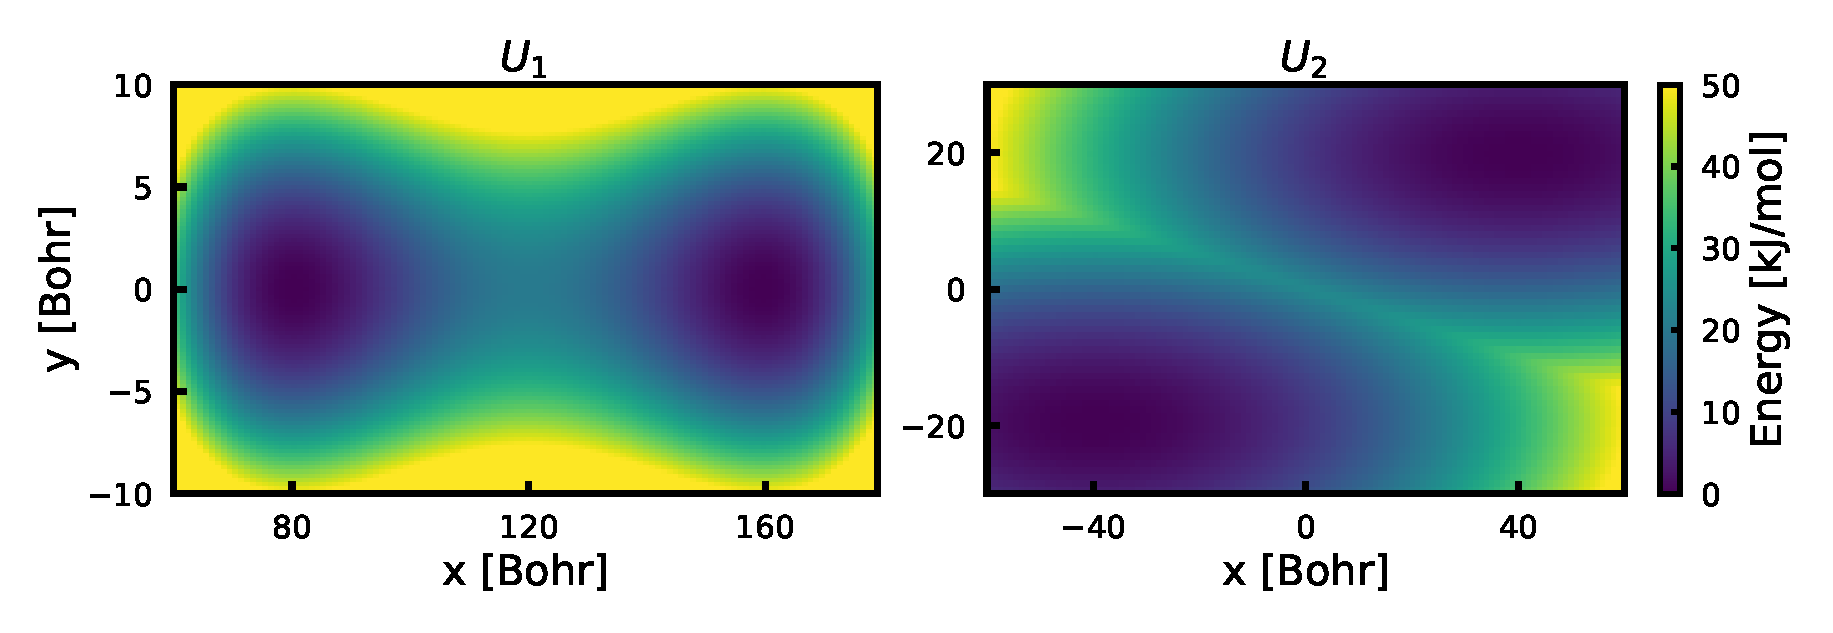
\includegraphics[width=1.0\textwidth]{bilder/U}
    \caption{Potentials for test calculations, Minima of $U_1$ are at located at (80,0) and (160,0). Minima of $U_2$ are located at (-40,-20) and (40,20). In both potentials two metastable states are separated by free energy barriers of roughly $20$~kJ/mol, which corresponds to 8~$k_B T$ at 300~K.}
\label{fig:potentials}%
\end{figure}
To simulate the particles dynamics a Velocity Verlet\autocite{swope1982computer} integrator was applied with a time step of 5~fs.
The initial momenta were drawn randomly from a Maxwell-Boltzmann distribution at 300~K.
Afterwards the temperature was controlled at 300~K by a Langevin thermostat\autocite{kroger2005models} with friction constant 0.001~fs$^{-1}$.
Crucial to the metastability of the system is the ratio of thermal energy~$k_B T$ to the barrier height.
Here, transition barriers of roughly 8~$k_B T$ (20~kJ/mol) was used.
Spontaneous transitions between minima in unbiased simulations can therefore be expected to be rare events.
All test simulation were completely performed in Python.
\newpage
\section{Molecular Dynamics Simulations}
\label{sec:comp MD}
For QM simulations a Python interface for the in-house program suite FermiONs++\autocite{kussmann2013pre,kussmann2017hybrid,laqua2018efficient} was used.
To generate starting structures for MD simulations minimum energy geometries were obtained with the FermiONs intern geometry optimizer.
Propagation of atomic coordinates with a Velocity Verlet\autocite{swope1982computer} integrator and temperature control with a Langevin thermostat\autocite{kroger2005models} (see algorithm~\ref{alg:ABM}) was done in Python.
For QM energy and gradient evaluation the PyFermiONsInterface was used.
All systems were simulated in vacuum.
MD simulations always consist of the following three steps:
\begin{enumerate}
  \item \textit{Heating}: Simulations were heated from 1~K to 300~K in 3000 time steps with a step size of 0.1~fs. Initial momenta were randomly drawn from a Maxwell-Boltzmann distribution. Velocities were rescaled every 10~time steps to increase the temperature by 1~K.
  \item \textit{Equillibration}: For thermal equilibration the heated system was simulated for at least 1.0~ps under application of the Langevin thermostat at 300~K with a friction coefficient of 0.001~fs$^{-1}$. The time-step was increased to 0.5~fs. To produce starting points for free energy estimation the system was also confined to the range of interest in CV space with harmonic walls.
  \item \textit{Production}: For production runs the equilibrated systems were simulated under additional application of one of the aforementioned enhanced-sampling algorithms.
\end{enumerate}

\subsection{Benchmark calculations}
Benchmark calculations for adaptive biasing force methods (section~\ref{sec:test}) were performed on Cl-F-ethane.
For this purpose PMFs for the transition between the gauge$^+$ and gauge$^-$ structure were calculated from 50~ps production MD runs on PBEh-3c/dev2-msvp\autocite{keal2005semiempirical} level of theory.
All calculation of PMFs from single trajectories were started in the gauge$^+$ structure.
To test convergence acceleration strategies additional second walkers were started in the gauge$^-$ structure.
Applied parameters for adaptive biasing algorithms are listed in table~\ref{tab:benchmark params} of the appendix for all simulations.
\newpage
\subsection{Illustrative Application to Reactions of Small Molecules}
To compare the performance of WTM-eABF with Umbrella Sampling a minimal model of the reactive center of Sirtuin 5 (Sirt5), which was already studied in a previous contribution of this group,\autocite{von2019finding} was used.
The S$_N$2 character of the reaction was captured by taking the difference of the O-C and C-N bond as reaction coordinate.
\begin{equation}
  \xi=d_{OC}-d_{CN}
\end{equation}
The starting geometry for MD simulations is given in figure~\ref{fig:cl-f-eth}.
\begin{figure}[H]
    \centering
    \includegraphics[width=0.4\textwidth]{bilder/cl-f-eth}
    \caption{Starting geometry for MD simulations of a minimal model system of the reactive center of Sirt5.}
\label{fig:cl-f-eth}%
\end{figure}
QM calculations of the positively charged system were performed on HF-3c/minix\autocite{sure2013corrected} level of theory.
In the real biochemical reaction in Sirt5, the two reactants are restricted in their freedom of movement by the surrounding protein. In order to achieve the same in this minimal model, the reactants are held on one line by harmonic potentials with a force constant of 1000~kJ/(mol\AA$^2$).
For Umbrella Sampling 25~ps trajectories were calculated in 22 windows along the reaction coordinate.
Starting structures were provided by a previously obtained minimum energy path.
WTM-eABF/CZAR simulations were performed in a single 50~ps trajectory.
For the WTM potential Gaussians of initial height $W=2$~kJ/mol and variance $\sigma_G=0.1$~\AA~were deposited every 10~fs.
The effective temperature was set to $\Delta T=4000$~K.
The fictitious particle was initialized with a mass of $m_\lambda=30$~a.u. and a thermal width of $\sigma_\lambda=0.05$~\AA.
To compare the convergence rate of PMFs obtained from Umbrella Sampling and WTM-eABF PMFs were calculated in fixed intervals from time trajectories with MBAR or CZAR, respectively.
The MBAR equation was solved self-consistently and considered converged, when the largest change of $\beta A_i$ was below 10$^{-7}$ and the norm of $\textbf{g}$, defined in eq.~\ref{eq:g}, was below 10$^{-4}$.
\newpage
As a second illustrative example for the application of WTM-eABF/CZAR the formation of deoxyadenosine was considered.
As reaction coordinate a linear combination of four bond length was applied:
\begin{equation}
  \xi = d_{CO} + d_{CC} + d_{OH1} - d_{OH2} \label{eq:CV ool}
\end{equation}
The product structure of the system is shown in figure~\ref{fig:cl-f-eth}.
\begin{figure}[H]
    \centering
    \includegraphics[width=0.4\textwidth]{bilder/ool_atoms}
    \caption{Molecular structure of deoxyadenosine. }
\label{fig:cl-f-eth}%
\end{figure}
QM calculations were performed on PBEh-3c/def2-msvp\autocite{keal2005semiempirical} level of theory.
For this purpose four 15~ps trajectories where simulated under application of shared-bias WTM-eABF/CZAR.
For the WTM potential Gaussians of initial height $W=1$~kJ/mol and variance $\sigma_G=0.1$~\AA~were deposited every 10~fs.
The effective temperature was set to $\Delta T=2000$~K.
The fictitious particle was initialized with a mass of $m_\lambda=15$~a.u. and a thermal width of $\sigma_\lambda=0.1$~\AA.

	\chapter{Results and Discussion}
\label{cha:results}
\section{Numerical Tests in an 2D Toy Potential}
\label{sec:2D}
As a simple test to check all ABM methods a single particle in the two-dimensional potential $U_2$ (eq.~\ref{eq:U2}) is considered.
By performing a simple 2D to 2D mapping in the absence of any dimensionality reduction, the analytical PMF and free energy difference is given by
\begin{equation}
  \begin{split}
    A(x,y)&=U_2(x,y) \\
    \Delta A_{A\to B} &= 0
  \end{split}
\end{equation}
The convergence of numerical PMFs and free energy differences to the analytical result with different adaptive biasing schemes (MtD, WTM, ABF, eABF and WTM-eABF) is computed over the course of 5~ns trajectories.
Note that all adaptive biasing methods depend on a different set of parameters.
Their convergence can therefore only be compared qualitatively.
A detailed analysis of the impact of the choice of parameters will be given in the following section.
Parameters applied in this section and resulting PMFs after 1, 3 and 5~ns are given in the Appendix.
In Fig.~\ref{fig:conv 2D} the convergence of the PMF and corresponding estimate for the free energy difference over time is given.
Fig.~\ref{fig:error 2D} shows remaining absolute local errors at the end of all simulations.

In an unbiased simulation the system stays trapped in one metastable state.
This is a example of quasi-nonergodic behavior, where simple time averages of MD trajectories do not converge to the correct ensemble average.
Because only a small region of CV space is explored the free energy difference $\Delta A_{A\to B}$ is highly overestimated.

All adaptive biasing methods reduce the metastability significantly and enable uniform sampling of both states.
In MtD/WTM simulations the PMF is given by a superposition of Gaussian hills, which are deposited linearly over time and fill both minima consecutively.
For this particular set of parameters no full convergence is reached in 5~ns.
Regions with high free energy at the margins remain unexplored due to incomplete filling of the PMF with Gaussians and the obtained PMFs deviate from the analytic result by about 20~\%.
However, using WTM this is intentional as the fraction of the PMF that is compensated in the simulation is chosen with the effective temperature $\Delta T$.
The height of Gaussians is reduced over time, which results in significantly smaller fluctuations and absolute errors of the PMF in large parts of the PMF than with MtD.
After 4~ns the free energy difference $\Delta A_{A\to B}$ obtained from WTM therefore converges safely towards 0~kJ/mol.
\begin{figure}[H]
   \centering
   \includegraphics[width=0.99\textwidth]{bilder/test_2D/conv}
   \caption{Convergence of free energy calculations with different adaptive biasing methods for a 2D to 2D mapping of toy potential $U_2$. On the right the RMSD between the analytical and numerical PMF is given over the course of 5~ns trajectories. On the right the development of free energy differences $\Delta A_{A\to B}$ given by eq.~\ref{eq:free energy diff} is shown. Both metastable states are separated by the line $0.25x+y$. Therefore $A$ includes all states $x>-4y$ and $B$ all states $x<-4y$, respectively.}
 \label{fig:conv 2D}%
\end{figure}
\begin{figure}[H]
  \centering
  \includegraphics[width=0.99\textwidth]{bilder/test_2D/error_5ns}
  \caption{Heat maps of the absolute difference between the analytic and numerical PMFs. Numerical PMFs are obtained from 5~ns MD trajectories at 300~K.}
\label{fig:error 2D}%
\end{figure}
With ABF after 3~ns the potential is mapped almost perfectly with maximum local errors below 1~kJ/mol. Also the RMSD of the PMF and free energy difference $\Delta A_{A\to B}$ converges rigorously to the analytic results.
For this particular example ABF force samples are simply given by the gradient of the analytical potential.
The variance of force samples, which is only introduced by the finite bin width, is therefore small and convergence of the ABF force in individual bins is reached almost instantly.
Even faster exploration of the PMF is only hindered by the ramp function, which is not strictly necessary for this toy example, but still applied to provide a more realistic test case for real chemical applications.
PMFs are obtained by thermodynamic integration of ABF forces with the FEM method, as shown in Fig.~\ref{fig:ti}.
\begin{figure}[H]
  \centering
  \includegraphics[width=0.99\textwidth]{bilder/test_2D/ti}
  \caption{On the left the convergence of the thermodynamic integration of ABF forces with the FEM method in a BFGS minimization is given for different time steps. On the right the mean local difference of optimized B-splines to the mean forces is shown.}
\label{fig:ti}%
\end{figure}
Convergence of the FEM method is reached reliably in 100 iterations by minimization of eq.~\ref{eq:RMSD} with the BFGS algorithm.
At the transition barrier, where the thermodynamic force changes rapidly, this introduces small errors to the PMF, which can be reduced with a smaller bin width and more B-spline functions.

Both eABF and WTM-eABF preserve the rigorous convergence behavior of ABF.
By estimating the thermodynamic force over the extended-system, the variance of obtained force samples depends on the harmonic force constant of the coupling of the fictitious to the physical particle.
For this toy example this introduces some noise to the mean force, where it would reduce said noise in real chemical applications.\autocite{lesage2017smoothed}
The PMF therefore shows small fluctuations of up to 2~kJ/mol for both methods and convergence to the true PMF is reached with a final RMSD of about 2~\%.
However, quite surprisingly convergence of the mean force with eABF is as fast as with ABF and WTM-eABF gives an additional speed up.
With WTM-eABF the estimate for the free energy difference stays close to 0~kJ/mol over the course of the hole simulation.
This indicates that the hole PMF is explored uniformly from the beginning and the system is never trapped in one state.

In this section the favorable convergence behavior of ABF, eABF and WTM-eABF was demonstrated.
In the following sections this methods will be discussed in further detail for a real chemical system with special focus on the influence of input parameters on the simulations.

\newpage
\section{Benchmark Calculations for the Torsion of Cl-F-Ethane}
\label{sec:test}
The following section will give a detailed discussion on the effect of different parameters on the time convergence of adaptive biasing force methods (ABF, eABF and WTM-eABF).
As test system the transition of the dihedral angle between the Cl- and F-group in Cl-F-Ethane from the gauge$^+$ ($60^\circ$) to the gauge$^-$ ($-60^\circ$) structure on the PBEh-3c/dev2-msvp level of theory in vacuum will be considered.

Figure~\ref{fig:ABF benchmark} shows PMFs obtained from ABF calculations with different values of $N_{full}$ in 50~ps trajectories and the time convergence of free energy differences and RMSD of the PMF in reference to the final ABF ($N_{full}=100$) result.
After roughly 30~ps all three PMFs converge to the same result within 1.0~\% deviation.
For high values of $N_{full}$ it takes longer to fill the ramp functions.
This delays diffusion to the second minimum and uniform sampling of the reaction coordinate.
Small values of $N_{full}$ are associated with a certain risk to drive the system away from thermal equilibrium at the beginning of the simulation.
As instantaneous force samples depend on all molecular coordinates, the variance of fluctuations in estimates of the mean force grows with the system size.
More specifically this fluctuations are dominated by high frequency terms due to bonded interactions\autocite{lesage2017smoothed}, which also leads to a dependence of the variance in ABF force samples on the amount of equillibration prior to the simulation.\autocite{blondel2004ensemble}
In this example the result are large fluctuations of $\Delta A$ over the course of the simulation.
Overall $N_{full}=100$ is found to result in a good compromise between fast and stable convergence of the PMF and free energy difference.
\begin{figure}[H]
    \centering
    \includegraphics[width=0.99\textwidth]{bilder/benchmark/ABF_benchmark_nfull}
    \caption{ABF benchmark}
    \label{fig:ABF benchmark}
\end{figure}
In eABF calculations mean square fluctuations $\sigma_F$ of force samples only depend on the spring force between the CV and extended variable and are inversely proportional to the thermal width $\sigma_\lambda$.
\begin{equation}
    \sigma_F^2 \propto \frac{k_\lambda}{\beta} = \frac{1}{\beta\sigma_\lambda}
\end{equation}
The choice of $\sigma_\lambda$ is therefore a trade-off between enhanced sampling of the CV by tight coupling to $\lambda$ and reduced fluctuations of the extended force.\autocite{lesage2017smoothed}
Figure~\ref{fig:conf eABF} shows both limiting cases.
With a small thermal width of $1^\circ$ convergence is hindered by high fluctuations of the mean force.
On the other hand for loose coupling to the fictitious particle ($N_{full}=20^\circ$) $\lambda$ is sampled uniformly, but the physical CV stays trapped in one metastable state.
The mass of the extended variable has much less influence on the resulting PMF.
If the mass of the fictitious particle is much smaller than that of the CV, it is more difficult to pull the CV over the TS and convergence is slowed down.
However, no consistent influence of $m_\lambda$ on the obtained PMF is observed.
Relatively large scattering in the estimates of $\Delta A$ from $-2$~kJ/mol to $2$~kJ/mol indicate that no full convergence is reached 50~ps.
To calculate $\Delta A$ the probability of finding the system in the gauge$^-$ or gauge$^+$ state is obtained by integrating the corresponding probability densities, which are separated at the maximum of the PMF.
Therefore, small fluctuations of the PMF at the TS can lead to large shifts of $\Delta A$, because the maximum of the PMF switches to different bins.
\begin{figure}[H]
  \centering
    \includegraphics[width=0.99\textwidth]{bilder/benchmark/eABF_benchmark_sigma}
    \includegraphics[width=0.99\textwidth]{bilder/benchmark/eABF_benchmark_mass}
   \caption{Convergence of eABF/CZAR with $m_\lambda=15$~a.u. and $N_{full}=100$.}
   \label{fig:conf eABF}
\end{figure}
Figure~\ref{fig:traj ABF} shows trajectories of simulations with ABF, eABF and WTM-eABF.
In WTM-eABF the number of transitions between both states is double as high is in a eABF normal ABF simulation with the same parameters of the extended-system.
This enables not only consistently faster convergence of the PMF, but also a more accurate result at the important TS region, as shown in Figure~\ref{fig:conf meABF}.
The fluctuations in the estimate of $\Delta A$ are therefore much smaller.
The WTM potential only enhances sampling by pushing the system to high free energy regions.
It has no significant impact on the resulting PMF, which is obtained from CZAR, as long the canonical ensemble is sampled.
WTM-eABF is therefore vary robust to the choice of WTM parameters like the Gaussian height $W$ and variance $\sigma_G$.
The influence of the eABF $m_\lamba$ and $\N_{full}$ is also even less severe, as both only impact enahanced sampling as well, which is always improved by the repulsive WTM potential.
\begin{figure}[H]
  \centering
    \includegraphics[width=0.99\textwidth]{bilder/benchmark/meta_eABF_benchmark_height}
    \includegraphics[width=0.99\textwidth]{bilder/benchmark/meta_eABF_benchmark_var}
   \caption{Convergence of WTM-eABF with $m_\lambda=5$~a.u., $\sigma_\lambda=5$, $\sigma_G=5$, $\tau_G=10$~fs, $\Delta T=2000$~K and $N_{full}=100$.}
   \label{fig:conf meABF}
\end{figure}
\begin{figure}[H]
     \centering
     \includegraphics[width=0.99\textwidth]{bilder/benchmark/ABF_trajs}
     \caption{Trajectories during ABF, eABF and WTM-eABF simulation.}
     \label{fig:traj ABF}
\end{figure}

\begin{figure}[H]
  \centering
    \includegraphics[width=0.99\textwidth]{bilder/benchmark/ABF_acc_benchmark}
   \caption{Convergence of ABF, eABF and WTM-eABF}
   \label{fig:conf ABF}
\end{figure}


% \begin{figure}[H]
%    \centering
%     \includegraphics[width=0.99\textwidth]{bilder/test_2D/ABF}  \\
%     \includegraphics[width=0.99\textwidth]{bilder/test_2D/eABF} \\
%     \includegraphics[width=0.99\textwidth]{bilder/test_2D/meta_eABF}
%     \caption{2D ABF, eABF and WTM-eABF test}
% \label{fig:2D ABF}%
% \end{figure}


\section{Application of WTM-eABF to S\textsubscript{n}2-Reactions}
\label{sec:Sn2}


\section{Ring Closing Reaction}
\label{sec:RCR}

\begin{figure}[H]
  \centering
    \includegraphics[width=0.99\textwidth]{bilder/results/R2_ool_results}
   \caption{Ring closing reaction}
   \label{fig:ool}
\end{figure}

	\chapter{Conclusion and Outlook}
\label{cha:conclusion}
Observing slow chemical reactions in molecular simulations still constitutes a enormous theoretical challenge.
Transitions between reactants are often rare events, that might happen on timescales far beyond what is computationally feasible.
In this thesis modern enhanced sampling algorithms, that enable diffusive behavior along reaction coordinates in short MD trajectories, are combined with highly efficient and accurate quantum-chemical methods in the in-house program package FermiONs++.
%The result is highly efficient importance-sampling of reaction coordinates, which enables the calculation of free energy curves on accurate quantum-chemical level of theory for a wide range of molecular processes.
Major strengths of the presented methods are:
\begin{enumerate}
  \item Uniform sampling of reaction coordinates in single trajectories of only few picoseconds,
  %\item faster convergence of free energy curves with the amount of sampled data,
  \item on-the-fly free energy estimates during the simulation for 1D reaction coordinates
  \item and the availability of a range of flexible strategies for parallelization that enable scaleable speedup.
\end{enumerate}
Especially promising is the application of ABF in an extended-Lagrangian based framework, where fictitious particles are coupled to CVs with harmonic potentials.
Together with CZAR, an asymptotically unbiased estimator for the free energy gradient, sampling acceleration is completely separated from free energy estimation.
This enables the combination of ABF with metadynamics to WTM-eABF/CZAR, a "working horse" algorithm, which stands out due to its wide applicability, robustness to input parameters and high efficiency.
Overall, by dramatically reducing the effort for the calculation of free energy curves this advances contribute towards making the calculation of free energy curves a routine tool in the characterization of chemical reactions.

However, even armed with enhanced-sampling strategies of utmost efficiency, considering that CVs selected from chemical intuition may not adequately describe the structural transformation at hand, free energy calculations can still fail by nonergodic sampling of orthogonal-space.
Additionally, if the collective variable does not include all slow degrees of freedom of a given transition, diffusion between reactant and product states might be hindered.
By applying multiple-walker strategies, like shared-adaptive biasing, this problem can be addressed by massive sampling though parallelisation.
Introducing replica-exchange (e.g., REX-WTM-eABF\autocite{fu2019taming}) promises further improvements by making high temperature configurations available to low temperature walkers and vice versa.
Another important direction of current research is the development of methods to improve or even completely automatize the selection of appropriate CVs, thus eliminating the intrinsic shortcoming of all CV based enhanced sampling algorithms.
For this purpose a variety of CV-discovery approaches were proposed, for example time-lagged independent component analysis (TICA)\autocite{perez2013identification}, autoencoders\autocite{reiter2019using} or deep machine learning\autocite{brandt2018machine,rydzewski2020multiscale}.
Another interesting approach for further improvement could be the combination of WTM-eABF with dynamically optimized CVs, which were already successfully applied for metadynamics.\autocite{brotzakis2018accelerating}


	\backmatter
	\pagenumbering{Roman}                    % romanische Nummerierung
	\sectionnumbering{Roman}
	\setcounter{page}{\theromanPagenumber}   % setzt die aktuelle Seitenzahl von vorne für die romanische Nummerierung fest

	\chapter{Appendix}
\label{cha:appendix}

\section{Definition of Collective Variables}
\label{sec:reaction coordinates}

In the present work distances, projected distances, angles and torsion angles between groups of atoms were used as collective variables for US, MtD, ABF, eABF or meta-eABF simulations.
Below analytic expressions for the calculation of all CVs, their gradients, inverse gradients and divergence of inverse gradients are given.

The center of mass $r^C$ of a group of $N$ atoms is calculated according to
\begin{equation}
  r^C(\textbf{x}) = \frac{1}{M^C} \sum_{i=0}^N m_i r_i
\end{equation}
with mass of each atom $m_i$ and Cartesian coordinates $r_i = (x_i,y_i,z_i)$. $M^C$ is the mass of the group.
All following collective variables are calculated between centers of mass. The index C will be dropped for convenience.
To obtain derivatives of single atoms the gradient its corresponding group is weighted with $m_i/M$.
The distances between group i and j is given by
\begin{equation}
 r_{ij} = r_j - r_i
\end{equation}
and the absolute distance is $d_{ij} = \| r_{ij}\|$.
The derivatives with respect to $r_i$ and $r_j$ are defined by
\begin{equation}
  \frac{\partial d_{ij}}{\partial r_j} = \frac{r_{ij}}{\|r_{ij}\|} = \hat{r}_{ij}
\end{equation}
\begin{equation}
  \frac{\partial d_{ij}}{\partial r_i} = - \hat{r}_{ij}
\end{equation}
where the hat denotes unit vectors.
The projection of distance $\| r_{ij}\|$ onto another axis $r_{jk}$ is defined by
\begin{equation}
  d^p_{ij} = r_{ij} \cdot \hat{r}_{jk}
\end{equation}
and the derivative of the projection is defined by
\begin{equation}
   \frac{\partial d^p_{ij}}{\partial r_i} = -\hat{r}_{jk}
\end{equation}
\begin{equation}
   \frac{\partial d^p_{ij}}{\partial r_j} = \hat{r}_{jk}
\end{equation}
The bond angle $\theta$ between three centers ($r_i, r_j, r_k$) is defined by the dot product of bond distances $r_{ji}$ and $r_{jk}$:
\begin{equation}
  \cos \theta = \hat{r}_{ji} \cdot \hat{r}_{jk}
\end{equation}
The gradient of $\theta$ is then given by
\begin{equation}
  \frac{\partial \theta}{\partial r_i} = \frac{(r_{ji} \times (r_{ji} \times r_{jk})) }{\| r_{ij}\| \| (r_{ji} \times (r_{ji} \times r_{jk})) \|}
\end{equation}
\begin{equation}
  \frac{\partial \theta}{\partial r_k} = \frac{(r_{kj} \times (r_{ji} \times r_{ji}))}{\| r_{kj}\| \| (r_{kj} \times (r_{ji} \times r_{ji})) \|}
\end{equation}
\begin{equation}
  \frac{\partial \theta}{\partial r_j}= -\frac{\partial \theta}{\partial r_i} - \frac{\partial \theta}{\partial r_k}
\end{equation}
The torsion angle $\phi$ between four Cartesian coordinates ($r_i, r_j, r_k, r_l$) is given by:
\begin{equation}
  \tan \phi = \frac{(\hat{r}_{ij} \times n_1) \cdot n_2}{n_1 \cdot n_2}
\end{equation}
with
\begin{equation}
  n_1 = r_{jk} - (r_{ij} \cdot \hat{r}_{jk})\hat{r}_{jk}
\end{equation}
\begin{equation}
  n_2 = r_{kl} - (r_{kl} \cdot \hat{r}_{jk})\hat{r}_{jk}
\end{equation}
The derivative of $\phi$ in Cartesian coordinates is given by:
\begin{equation}
  \frac{\partial\phi}{\partial r_i} = - \frac{\hat{r}_{ji}\times\hat{r}_{jk}}{\|r_{ij}\|\sin^2\theta_{ijk}}
\end{equation}
\begin{equation}
  \frac{\partial\phi}{\partial r_l} = - \frac{\hat{r}_{kl}\times\hat{r}_{jk}}{\|r_{kl}\|\sin^2\theta_{jkl}}
\end{equation}
\begin{equation}
  \frac{\partial\phi}{\partial r_j} = \bigl(\frac{\|r_{ij} \| \cos\theta_{ijk}}{\|r_{jk} \|}-1\bigr) \frac{\partial\phi}{\partial r_i} - \bigl( \frac{\|r_{kl} \| \cos\theta_{jkl}}{\|r_{jk} \|}\bigr)\frac{\partial\phi}{\partial r_l}
\end{equation}
\begin{equation}
  \frac{\partial\phi}{\partial r_k} = - \frac{\partial\phi}{\partial r_i} - \frac{\partial\phi}{\partial r_l} - \frac{\partial\phi}{\partial r_j}
\end{equation}
where $\partial \phi/\partial r_j$ and $\partial \phi/\partial r_k$ are defined to fulfill the conservation of (angular) momentum.

Always choosing as inverse gradient $\textbf{v}(\xi) = \nabla \xi/\|\nabla \xi \| ^2$ the divergence of vector fields $\textbf{v}_i(\xi)$ are given by
\begin{equation}
  \nabla \cdot \textbf{v}(d) = \frac{2}{d},
\end{equation}
\begin{equation}
  \nabla \cdot \textbf{v}(d^p) = 0,
\end{equation}
\begin{equation}
  \nabla \cdot \textbf{v}(\theta) = \cot \theta,
\end{equation}
\begin{equation}
  \nabla \cdot \textbf{v}(\phi) = 0,
\end{equation}
for distances, projected distances, angles and dihedrals, respectively.

\section{Numerical Examples}
\label{sec:num examples}

To test adaptive biasing methods the 2D test potentials $U_1$ and $U_2$ were used. For numerical tests of adaptive biasing methods a particle with a mass of 10~a.u. is simulated according to Algorithm \ref{alg:ABM} with a step size of 5 fs and at a temperature of 300~K.
\begin{equation}
  U_1(x,y) = a(x-c)^2(x+d)^2 + by^2 \label{eq:U1}
\end{equation}
\begin{equation}
  U_2(x,y) = -\ln\bigl( e^{-a(x-c)^2 - b(y-d)^2} + e^{-a(x+c)^2 - b(y+d)^2} \bigr) \label{eq:U2S}
\end{equation}
\begin{table}[H]
        \centering
        \caption{Free Parameters for definition of $U_1$ and $U_2$.}
        \begin{tabular}{ c | c  c  c  c }
                & a & b & c & d   \\
                \hline
                $U_1$  & $8.0e-6$ kJ/mol & $0.5$ kJ/mol & 80 Bohr & 160 Bohr \\
                $U_2$  & $0.005$ kJ/mol  & $0.040$ kJ/mol & 40 Bohr & 20 Bohr \\
        \end{tabular}
        \label{tab:2D pots}
\end{table}

\begin{figure}[H]
    \centering
    \vspace{-1cm}
    \subfloat[$U_1$]{{\includegraphics[width=0.49\textwidth]{bilder/U1} }}
    \subfloat[$U_2$]{{\includegraphics[width=0.49\textwidth]{bilder/U2} }}
    \caption{Potentials for test calculations}
\label{fig:potentials}%
\end{figure}

	\appendix
	\listoftables
	\listoffigures

%   \nocite{*}								 % auch Quellen die nicht verwendet wurden tauchen in Literaturverzeichnis auf
	\inputencoding{utf8}
	\printbibliography[title=Bibliography]   % Literaturverzeichnis

\end{document}
